\documentclass[lettersize,journal]{IEEEtran}
% code

\hyphenation{op-tical net-works semi-conduc-tor IEEE-Xplore}
\def\BibTeX{{\rm B\kern-.05em{\sc i\kern-.025em b}\kern-.08em
T\kern-.1667em\lower.7ex\hbox{q}\kern-.125emX}}
% \usepackage{balance}
\input{dding_template/tex_packages/tex_packages_general.tex}
\input{dding_template/tex_macros/tex_macros_general.tex}

\newcommand*{\sat}{\mathcal{S}}
\newcommand*{\fe}{\mv r}
\newcommand*{\ptfrac}[2]{\tfrac{\partial #1}{\partial #2}}
\newcommand*{\dtfrac}[2]{\tfrac{\der #1}{\der #2}}
\newcommand*{\q}{\mv q}
\newcommand*{\dq}{\dot{\mv q}}
\newcommand*{\ddq}{\ddot{\mv q}}
\newcommand*{\qd}{\mv q_d}
\newcommand*{\dqd}{\dot{\mv q_d}}
\newcommand*{\ddqd}{\ddot{\mv q_d}}

\newcommand*{\NN}{\mv\Phi}
\newcommand*{\act}{\mv\phi}
\newcommand*{\wth}{\mv\theta}
\newcommand*{\wV}{\mm V}

\begin{document}
\title{
Constrained Optimization-Based Neuro-Adaptive Control (CoNAC) for Uncertain Euler-Lagrange Systems Under Weight and Input Constraints 
%Constrained Optimization-Based neuro-Adaptive Control (CoNAC) for Uncertain Euler-Lagrange Systems With Input Constraints/
}

\markboth{IEEE TRANSACTIONS ON NEURAL NETWORKS AND LEARNING SYSTEMS,
~Vol.~00, No.~0, Month~2024
}%
{How to Use the IEEEtran \LaTeX \ Templates}

\maketitle

\begin{abstract}
    This study presents a constrained optimization-based neuro-adaptive controller (CoNAC) for uncertain Euler-Lagrange systems subject to weight norm and input constraints. A deep neural network (DNN) is employed to approximate the ideal stabilizing control law, compensating for lumped system uncertainties while addressing both types of constraints. The weight adaptation laws are formulated through a constrained optimization problem, ensuring first-order optimality conditions at steady state. The controller's stability is rigorously analyzed using Lyapunov theory, guaranteeing bounded tracking errors and DNN weights. Numerical simulations comparing CoNAC with three benchmark controllers demonstrate its effectiveness in tracking error regulation and satisfaction of constraints.
\end{abstract}

\begin{IEEEkeywords}
Neuro-adaptive control, constrained optimization, deep neural network, Euler-Lagrange system, input constraint.
\end{IEEEkeywords}

%  SECTION INTRODUCTION ===================================
\section{Introduction}

\subsection{Background}

\IEEEPARstart{M}{any} engineering systems, including those in aerospace, robotics, and automotive applications, can be modeled using Euler-Lagrange systems. These systems are governed by dynamic equations derived from energy principles and describe the motion of mechanical systems with constraints. In practice, however, such systems often exhibit uncertainties due to unmodeled dynamics, parameter variations, or external disturbances. These uncertainties can significantly degrade control performance and, in some cases, lead to instability. To address these challenges, adaptive control methods have been widely employed to ensure robust performance in the presence of system uncertainties \cite{RN4}, \cite{RN2}.

More recently, neuro-adaptive control approaches have been introduced to approximate unknown system dynamics or entire control laws using neural networks (NNs) \cite{RN1}. NNs are well-known for their universal approximation property, which allows them to approximate any smooth function over a compact set with minimal error. Various types of NNs have been utilized in neuro-adaptive control, including simpler architectures like single-hidden layer (SHL) neural networks \cite{RN29}, \cite{RN44} and radial basis function (RBF) neural networks \cite{RN26}, \cite{RN10}, as well as more complex models like deep neural networks (DNNs) \cite{RN16} and their variations. SHL and RBF NNs are often employed to approximate uncertain system dynamics or controllers due to their simplicity \cite{RN44, RN56, RN3, RN41}, while DNNs offer greater expressive power, making them more effective for complex system approximations \cite{RN25}. Additionally, variations of DNNs, such as long short-term memory (LSTM) networks for time-varying dynamics \cite{RN14} and physics-informed neural networks (PINNs) for leveraging physical system knowledge \cite{RN15}, have further extended the capabilities of neuro-adaptive control systems.

A critical aspect of neuro-adaptive control is the weight adaptation law, which governs how NN parameters are updated. Most studies derived these laws using Lyapunov-based methods, ensuring the boundedness of the tracking error and weight estimation error, thus maintaining system stability under uncertainty.

However, two significant challenges persist in using NNs for adaptive control. First, the boundedness of NN weights is not inherently guaranteed, which can result in unbounded outputs. When NN outputs are used directly in the control law, this may lead to excessive control inputs, violating input constraints. Such constraints are commonly encountered in industrial systems, where actuators are limited by physical and safety requirements in terms of amplitude, rate, or energy \cite{RN18}. Failing to address these constraints can degrade control performance or even destabilize the system.

Therefore, addressing these two key issues—ensuring weight boundedness and satisfying input constraints—is essential for the reliable design of neuro-adaptive controllers. The following section will provide a detailed review of the existing solutions to these challenges.

\subsection{Literature Review}

\subsubsection{Ensuring Weight Norm Boundedness}

A common challenge in neuro-adaptive control is maintaining the boundedness of the NN weights to ensure stability. In many studies, projection operators were employed to enforce upper bounds on the weight norms, ensuring that the weights do not grow unboundedly. For example, in \cite{RN16, RN14, RN11}, projection operators were used to constrain the weight norms to remain below predetermined constants. However, these constants were often selected as large as possible due to the lack of theoretical guarantees regarding the global optimality of the weight values. While this approach ensured that the NN remained stable, it did not necessarily result in optimal performance.

In addition to projection operators, some studies utilized modification techniques like $\sigma$-modification \cite{RN10} and $\epsilon$-modification \cite{RN41, RN3}. These methods ensured that the NN weights remained within an invariant set by incorporating stabilizing functions into the adaptation law. Although these techniques were effective in ensuring boundedness and avoiding weight divergence, they similarly lacked a formal analysis of the optimality of the adapted weights, leaving room for improvement in terms of performance optimization.

\subsubsection{Satisfying Input Constraints}

The second major issue is satisfying input constraints, particularly in systems where actuators are subject to physical limitations. The unpredictable outputs of NNs can sometimes lead to excessively large control inputs, violating these constraints. This problem is exacerbated in neuro-adaptive controllers that attempt to cancel out system dynamics using conventional methods like feedback linearization or backstepping. In such cases, controllers may produce overly aggressive control inputs, even when the system's natural dynamics are stabilizing, leading to unnecessary saturation of the control inputs.

To address input saturation, many studies introduced auxiliary systems. These systems mitigated the effects of control input saturation by modifying the control strategy when saturation occurred. For instance, in \cite{RN55, RN56, RN3}, auxiliary states were generated whenever input saturation was detected, and these states were incorporated into the adaptation law to adjust the NN weights accordingly. This approach helped the controller reduce input saturation by indirectly regulating the auxiliary states.

Alternatively, auxiliary states can also be used as feedback terms in the control law to directly compensate for the effects of input saturation constraints, as demonstrated in \cite{RN34, RN38, RN37}. In \cite{RN41}, the NN was used to approximate the desired control input, compensating for input saturation. However, these approaches typically handle input bound constraints on a per-input basis (\ie applying bounds to each scalar control variable individually), and may not account for more complex, nonlinear constraints, like input norm constraints, which are commonly found in physical systems such as robotic actuators or motor systems.

\subsubsection{Limitations of Existing Approaches and Potential of Constrained Optimization}

Although both the projection operator methods for weight norm boundedness and the auxiliary system approach for input constraints have shown effectiveness, they come with significant limitations. Projection operators and modification techniques do not guarantee the optimality of the adapted weights. Moreover, auxiliary systems typically handle only simple forms of input constraints, such as input bound constraints, limiting their ability to address more complex, nonlinear constraints like input norm constraints.

To overcome these limitations, constrained optimization offers a promising approach. By formulating the neuro-adaptive control problem as an optimization problem with constraints, it is possible to adapt the NN weights while minimizing an objective function (e.g., tracking error) subject to both weight norm and input constraints. Constrained optimization provides a theoretical framework for defining optimality and presents numerical methods for finding solutions that satisfy the constraints \cite{RN22}.

In existing literature, constrained optimization techniques, such as the Augmented Lagrangian Method (ALM) \cite{RN60} and the Alternating Direction Method of Multipliers (ADMM) \cite{RN58, RN59}, have been used to train NNs offline. These methods impose constraints to address issues like gradient vanishing in backpropagation. However, to the best of the authors' knowledge, no prior work has applied constrained optimization to adaptive control systems with real-time weight adaptation. This gap suggests that constrained optimization could be key to addressing both weight norm boundedness and input constraints in a unified, theoretically grounded framework, particularly in real-time neuro-adaptive control.

\subsection{Contributions}

The main contributions of this study are listed as follows:
\begin{itemize}
    \item A constrained optimization-based neuro-adaptive controller (CoNAC) is developed using a DNN, where input constraints and the boundedness of NN weights are formulated as inequality constraints within the adaptation process.
    \item The weight adaptation laws in CoNAC are derived using constrained optimization theory to minimize the objective function while satisfying the inequality constraints. The adaptation laws ensure convergence of the weights to the first-order optimality conditions, specifically the Karush-Kuhn-Tucker (KKT) conditions.
    \item The forward sensitivity method is applied in CoNAC to accurately calculate the gradient of the objective function.
    %, enabling more precise real-time adaptation.
\end{itemize}

\subsection{Organization}

The remainder of this paper is organized as follows. 
Section \ref{sec: Problem Formulation} presents the target system and control objective.
Section \ref{sec:ctrl design} introduces the proposed controller and the architecture of DNN in the controller. 
In Section \ref{sec:adap_laws}, the weight adaptation laws are developed.
Candidates of the weight and input constraints are presented in Section \ref{sec:cstr candidates}.
Section \ref{sec:stability} analyzes the stability of the proposed controller.
A comparative study of the four selected controllers, including the proposed controller, is reported in Section \ref{sec:sim}.
Finally, Section \ref{sec:conclusion} concludes the paper and discusses potential future work.
% The appendices provide the proof of the lemma used in the stability analysis.

%  SECTION PROBLEM FORMULATION ============================
\section{Problem Formulation}\label{sec: Problem Formulation}

\subsection{Notation}
In this study, the following notation is used:

\begin{itemize}
    \item $\otimes$ denotes the Kronecker product \cite{RN17}.
    \item $\mv x=[x_i]_{i\in[1,\cdots,n]}\in\R^n$ and $\mm A\triangleq [a_{ij}]_{i\in[1,\cdots,n],j\in[1,\cdots ,]}\in\R^{n\times m}$ denotes a vector and a matrix.
    % \item $x_{(i)}$ denotes the $i\textsuperscript{th}$ element of the vector $x\in\mathbb R^n$.    
    % \item $A_{(i,j)}$ is the $i\textsuperscript{th}$ row-$j\textsuperscript{th}$ column element of matrix $A$.
    \item $\text{row}_i(A)$ denotes the $i\textsuperscript{th}$ row of the matrix $A\in\R^{n\times m}$. 
    % \item $\text{col}_i(A)$ and $\text{row}_j(A)$ denote the $i\textsuperscript{th}$ column and $j\textsuperscript{th}$ row of $A\in\R^{n\times m}$, respectively.
    \item $\textit{vec}(A)\triangleq [\text{row}_1(A^\top)  ,\cdots,\text{row}_m(A^\top)  ]^\top   $ for $A\in\R^{n\times m}$.
    % \item $\textit{vec}(A)\triangleq [\text{col}_1(A)^\top  ,\cdots,\text{col}_m(A)^\top  ]^\top   $ for $A\in\R^{n\times m}$.
    \item $\lambda_\text{min}(A)$ denotes the minimum eigenvalue of the matrix $A\in\R^{n\times n}$.
\end{itemize}

\subsection{Model Dynamics and Control Objective}

Consider an uncertain Euler-Lagrange system modeled as
\begin{equation}
    \mm M\ddq + \mm V_m + \mm F + \mm G + \mv\tau_d
    =
    \sat(\mv\tau)
    \label{eq:sys1}
\end{equation}
where $\q\in \R^n$ denotes the generalized coordinate, $\mv \tau_d$ represents disturbance and $\mv\tau\in\R^n$ denotes the control input. 
The terms $\mm M\triangleq\mm M(\q)\in\R^{n\times n}$, $\mm V_m\triangleq\mm V_m(\q,\dq)\in\R^{n\times n}$, $\mm F\triangleq\mm F(\dq)\in\R^{n}$ and $\mm G\triangleq\mm G(\q)$ represent the unknown inertia matrix, Coriolis/centripetal matrix, friction terms and gravity vector
The function $\sat(\cdot):\R^n\to\R^n$ represents the inherent physical limitations of the actuators and is defined as 
\begin{equation}
    \sat(\mv\tau)
    \triangleq
    \begin{cases}
        \mv\tau, 
        & 
        \text{if } \Vert\mv\tau\Vert\le \bar\tau,
        \\
        \bar\tau
        \cdot
        \tfrac{\mv\tau}{\Vert\mv\tau\Vert}, 
        & 
        \text{otherwise},
    \end{cases}
\end{equation}
where $\bar\tau$ denotes the maximum norm of control input.
To account for these limitations, it is essential to incorporate physically motivated constraints into the controller design.
Section \ref{sec:cstr candidates} introduces candidate constraints that can be applied to ensure compliance with these physical limitations.

The Euler-Lagrange system \eqref{eq:sys1} satisfy some important physical properties \cite[see, Chap. 3 Tab. 3.2.1]{Lewis:1998aa}.
We introduce the following properties:
\begin{prop} \cite{Lewis:1998aa}
    The inertia matrix $\mm M$ is symmetric, positive definite and bounded.
    \label{prop:M}
\end{prop}

\begin{prop} \cite{Lewis:1998aa}
    The Coriolis/centripetal matrix $\mm V_m$ can always be selected so that the matrix $\dot{\mm M}-2\mm V_m$ is skew-symmetric.
    \label{prop:skew}
\end{prop}

\begin{prop}
    The disturbance $\mv\tau_d$ is bounded so that $\norm{\mv\tau_d}\le \bar\tau_d$.
\end{prop}

In conclusion, the control objective is to develop a neuro-adaptive controller that enables $\q$ to track a continuously differentiable desired trajectory $\qd(t): \R \to \R^n$, compensating for the external disturbance while addressing the imposed constraints.
Considering the control input saturation function, $\qd(t)$ is supposed to be available to design a feasible control input in the presence of the control input saturation.

%  SECTION CONTROLLER DESIGN ==============================
\section{Control Law Development}\label{sec:ctrl design}

The architecture of the proposed CoNAC is illustrated in Fig.~\ref{fig: controller}, consisting of: a DNN that functions as a neuro-adaptive controller, and a weight optimizer for the DNN. 
Section \ref{sec:NAC} presents the neuro-adaptive controller along with the reference generator, and Section \ref{NN definition} defines the DNN model. The weight optimizer will be detailed in Section \ref{sec:adap_laws}.

\begin{figure*}[!t]
    \centering
    \includegraphics[width=0.7\linewidth]{fig/Controller.drawio.png}
    % \includesvg[width=0.75\linewidth]{Controller.drawio.svg}
    \caption{Architecture of the constrained optimization-based neuro-adaptive controller (CoNAC).}
    \label{fig: controller}
\end{figure*}

\subsection{Neuro-Adaptive Controller Design}\label{sec:NAC}

First, let us define the filtered tracking error $\fe\in\R^n$ as 
\begin{equation}
    \fe \triangleq \dot{\mv e}-\mm\Lambda \mv e
    ,
    \label{eq:err:filtered}
\end{equation}
where $\mv e \triangleq \q - \qd$ denotes the tracking error, $\dot{\mv e} \triangleq \dq - \dqd$ represents the derivative of the tracking error, and $\mm\Lambda\in\R^{n\times n}$ is a user-designed positive definite matrix.
Since \eqref{eq:err:filtered} is stable system, it implies that $\mv e$ is bounded if $\fe$ is bounded.

Using $\fe$, the system dynamics \eqref{eq:sys1} can be rewritten as
\begin{equation}
    \mm M \dot\fe
    =
    -\mm V_m \fe
    -\mm K \fe
    + \mv f
    -\mv \tau_d + \sat(\mv\tau)
    ,
\end{equation}
where $\mm K\in\R^{n\times n}$ denotes arbitrary symmetric positive definite matrix and $
    \mv f\triangleq \mv f(\q,\dq,\dqd,\ddqd)
    =
    \mm K \fe
    +\mm M(-\ddqd+\mm\Lambda\dot{\mv e})
    +
    \mm V_m(-\dqd+\mm\Lambda\mv e)
    -
    \mm F
    -
    \mm G
    \in\R^n
$ denotes the lumped system uncertainty.

Consider the Lyapunov function $\mathcal V_1\triangleq \tfrac{1}{2}\fe^\top \mm M\fe$. 
Invoking Property \ref{prop:skew}, the time derivative of $\mathcal V_1$ is
\begin{equation}
    \begin{aligned}
        \dot{\mathcal V}_1
        =&
        \fe^\top \mm M (
            -\mm V_m \fe -\mm K \fe + \mv f
            -\mv \tau_d + \sat(\mv\tau)
        )
        +
        \tfrac{1}{2}
        \fe^\top \dot{\mm M}\fe
        \\
        =&
        -
        \fe^\top \mm K \fe 
        +
        \fe^\top (
            \mv f+\sat(\mv\tau)
            -\mv \tau_d
        )
        +
        \tfrac{1}{2}
        \fe^\top(\dot{\mm M}- 2\mm V_m)\fe
        \\
        \le&
        -\lambda_\text{min}(\mm K)\norm{\fe}^2
        +
        \bar\tau_d\norm{\fe}
        +
        \fe^\top (\mv f+\sat(\mv \tau))
        \\
        \le&
        -\lambda_\text{min}(\mm K)\norm{\fe}^2
        +
        \bar\tau_d\norm{\fe}
        +
        \fe^\top (\sat(\mv\tau)-\mv\tau^*)
        ,
    \end{aligned}
    \label{eq:lya1:dot1}
\end{equation}
where $\mv\tau^*\triangleq -\mv f$ is the ideal control input. 
Therefore, one can conclude that $\fe$ is exponentially stable so that $\lim_{t\to\infty}\norm{\fe}=\tfrac{\bar\tau_d}{\lambda_\text{min}(\mm K)}$, if $\mv \tau=-\mv\tau^*$ can be realized.
However, $\mv \tau^*$ is not available in practice, since $\mv f$ is unknown.

To overcome this issue, a DNN is employed to approximate $\mv\tau^*$.
Let $\NN\triangleq\NN(\q_{NN};\wth): \R^{l}\times\R^{\Xi}\to\R^{n}$ represent the DNN, where $\q_{NN}\in\R^{l}$ is the DNN input vector, and $\wth\in\R^{\Xi}$ is the vector of trainable weights.
The architecture of $\NN(\q_{NN};\wth)$ will be defined in Section \ref{NN definition}.
According to the universal approximation theorem for DNNs \cite{RN33}, $\NN(\q_{NN};\wth)$ can approximate a nonlinear function $\mv g(\cdot)$ with an ideal weight vector $\wth^*$ on a compact subset $\Omega_{NN}\in\R^{l}$ to $\mv\epsilon$-accuracy, such that $\sup_{\q_{NN}\in\Omega_{NN}}\norm{ \NN(\q_{NN};\wth^*) - \mv g(\cdot)} = \mv\epsilon < \infty$.
Furthermore, the theorem states that the norm of $\wth^*$ is bounded, \ie $\norm{\wth^*}\le \bar\wth<\infty$.
In this study, $\wth^*$ is defined as a local optimal point, rather than a global optimal point.

In conclusion, the ideal control law $\mv\tau^*$ is expressed by the DNN approximation with the ideal weight vector $\NN^*\triangleq\NN(\q_{NN};\wth^*)$ as follows:
\begin{align}
    \mv\tau^*=& -(\NN^*+\mv\epsilon),
    \label{eq:control:ideal}
\end{align}
which is estimated online by
\begin{align}
    \mv\tau =& -\hat\NN,
    \label{eq:control:est}
\end{align}
where $\hat\NN\triangleq\NN(\q_{NN};\hat\wth)$, and  $\hat\wth$ is the estimated weight vector for $\wth^*$.

Substituting \eqref{eq:control:ideal} and \eqref{eq:control:est} into \eqref{eq:lya1:dot1}, the time derivative of $\mathcal V_1$ can be rewritten as
\begin{equation}
    \dot{\mathcal V}_1
    \le 
    -\lambda_\text{min}(\mm K)\norm{\fe}^2
    +
    \bar\tau_d\norm{\fe}
    +
    \fe^\top (\sat(\hat\NN)-\NN^*-\mv\epsilon)
    .
    \label{eq:lya1:dot2}
\end{equation}
Finally, one can conclude that the result of \eqref{eq:lya1:dot1} can be obtained by adapting $\hat\wth$ to $\wth^*$ (\ie $\hat\NN\to\NN^*$).

\subsection{Deep Neural Network (DNN) Model}\label{NN definition}

The DNN architecture $\NN_k = \NN(\q_{NN};\wth)$ can be recursively represented as follows:
\begin{equation}
    \NN_i \triangleq
    \begin{cases}
        \wV_i^\top \NN_i(\NN_{i-1}), 
        &
        i\in[1,\dots,k],
        \\
        \wV_0^\top \q_{NN},
        &
        i=0
        ,
    \end{cases}
    \label{eq. DNN structure 2}
\end{equation}
where $\wV_i\in\R^{(l_i+1)\times l_{i+1}}$ is the weight matrix of the $i\textsuperscript{th}$ layer, and $\act_i: \R^{l_i}\to\R^{l_i+1}$ represents the activation function of the $i\textsuperscript{th}$ layer. 
The activation function is defined as $\act_i(\mv x)=[\sigma(x_1),\sigma(x_2),\cdots, \sigma(x_{l_{i}}), 1]^\top,\ \forall\mv x\in\R^{l_i}$, where $\sigma: \R\to\R$ is a nonlinear function, and the augmentation of $1$ is used to account for bias terms in the weight matrices. 
Notice that the output size of $\NN(\cdot)$ is the same as that of the control input $\mv\tau$ (\ie $l_{k+1}=n$). 


One of the widely used activation functions for large DNNs is from the ReLU family \cite{RN27}, which effectively avoids the gradient vanishing problem during error backpropagation. 
However, for control applications, where relatively shallow DNNs are typically sufficient and the gradient vanishing issue is less severe, the sigmoid function or the hyperbolic tangent function is commonly used as the activation function. 
These functions simplify stability analysis due to their continuous differentiability, and their outputs and gradients satisfy $\norm{\act_i(\mv x)} < \infty$ and  $\norm{\dtfrac{\act_i(\mv x)}{\mv x}}_F < \infty,\ \forall\mv x\in\R^{l_i}$. 
In this study, the hyperbolic tangent function $\tanh(\cdot)$ was selected as the activation function (\ie $\sigma(x) = \tanh(x)),\ \forall x\in\R$, which provides desirable boundedness with $\norm{\sigma(x)}<1$ and $\norm{\dtfrac{\sigma(x)}{x}}< 1$.

For simplicity, each layer's weights are vectorized as $\wth_i\triangleq\textit{vec}(\wV_i)\in\R^{\Xi_i}$, where $\Xi_i\triangleq (l_i+1)l_{i+1}$ is the number of weights in the $i\textsuperscript{th}$ layer. 
The total weight vector $\wth\in\R^{\Xi}$ is defined by augmentating $\wth_i$ for all $i\in \left[0,\cdots,k\right]$ as 
\begin{equation}
    \wth \triangleq 
    \begin{bmatrix}
        \wth_k\\
        \wth_{k-1}\\
        \vdots\\
        \wth_0
    \end{bmatrix}
    =
    \begin{bmatrix}
        \textit{vec}(\wV_k)\\
        \textit{vec}(\wV_{k-1})\\
        \vdots\\
        \textit{vec}(\wV_0)
    \end{bmatrix},
\end{equation}
where $\Xi={\sum_{i=0}^{k} \Xi_i}$ represents the total number of weights. The gradient of $ \NN(\q_{NN};\wth)$ with respect to $\wth$ is defined as
\begin{equation}
    \ptfrac{\NN}{\wth}=
    \begin{bmatrix}
        \ptfrac{\NN}{\wth_k}&
        \ptfrac{\NN}{\wth_{k-1}}&
    \cdots &
        \ptfrac{\NN}{\wth_0}
    \end{bmatrix}
    \in\R^{n \times \Xi}
    \label{eq. nabla phi}
\end{equation}
where
\begin{equation}
    \ptfrac{\NN}{\wth_i} = 
    \begin{cases}
        (\mm I_{l_{k+1}}\otimes \act_{k}^\top  ), 
        &
        i=k 
        \\
        \wV_k^\top   \act_{k}' (\mm I_{l_{k}}\otimes  \act_{k-1}^\top  ), 
        & 
        i=k-1
        \\
        &
        \vdots 
        \\
        \wV_k^\top   \act'_{k} \cdots \wV_1^\top  \act_1' (\mm I_{l_1}\otimes \q_{NN}^\top  ), 
        &
        i = 0
    \end{cases},
\end{equation}
where $\act_i\triangleq \act_i(\NN_{i-1})$ and $\act_i'\triangleq \ptfrac{\act_i}{\NN_{i-1}}$.

In the following sections, let $\NN^*_i$ represent the output of the $i\textsuperscript{th}$ layer with the ideal weight vector $\wth^*$. 
Additionally, define $\act^*_i\triangleq\act_i(\NN^*_{i-1})$ and $\act^{*'}_i\triangleq \ptfrac{\act^*_i}{\NN^*_{i-1}}$. 
Similarly, $\hat\NN_i$ denotes the output of the $i\textsuperscript{th}$ layer with the estimated weight vector $\hat \wth$, and define $\hat\act_i\triangleq\act_i(\hat\NN_{i-1})$ and $\hat\act_i'\triangleq \ptfrac{\hat\act_i}{\hat\NN_{i-1}}$, respectively.

%  SECTION ADAPTATION LAW DERIVATION =======================
\section{Weight Adaptation Laws}\label{sec:adap_laws}

% \subsection{Adaptation Law using Lagrangian Function}
\subsection{Weight Optimizer Design}

Consider a positive definite objective function defined as 
\begin{equation}
    J(\fe;\hat\wth)\triangleq 
    \tfrac{1}{2} \fe^\top  \mm W\fe
\end{equation}
where $\mm W\in\R^{n\times n}$ is symmetric positive weighting matrix.
Inequality constraints $c_j,\ j\in\mathcal{I}$, are imposed during the weight adaptation process to minimize the objective function, where $\mathcal I$ denotes the set of the imposed inequality constraints. 
The corresponding constrained optimization problem is formulated as
\begin{equation}
    \begin{matrix}
        \min_{\hat\wth} \ J(\fe;\hat\wth)
        \\ \\
        \begin{aligned}
        \text{s.t. }&c_{j}(\hat\wth) 
        \le0, \quad j\in\mathcal{I},
        \end{aligned}
    \end{matrix}
    \label{eq. train obj}
\end{equation}
Here, $\fe$ is considered a pre-defined data or parameter for this optimization problem. The Lagrangian function is defined as
\begin{equation}
    L(
        \fe,\hat\wth,[\lambda_j]_{j\in\mathcal I}
    ) 
    \triangleq 
    J(\fe;\hat\wth) 
    + 
    \sum_{j\in\mathcal I}
    \lambda_{j}
    c_{j}(\hat\wth)
\end{equation}
where $\lambda_j$ denotes the Lagrange multiplier for each constraint.

The adaptation laws for $\hat\wth$ and $[\lambda]_{j\in\mathcal I}$ are derived to solve the dual problem of \eqref{eq. train obj} (\ie  $\min_{\hat\wth} \max_{[\lambda]_{j\in\mathcal I}}L(\fe,\hat\wth,[\lambda]_{j\in\mathcal I})$), as follows:
\begin{subequations}
    \begin{align}
            \dot {\hat\wth}&=-\alpha {\partial L\over\partial \hat\wth}
            =-\alpha 
            \bigg(
            {\partial J\over \partial \hat\wth}+\sum_{j\in\mathcal{I}}
            \lambda_j {\partial c_j\over\partial \hat\wth}
            \bigg),
        \label{eq. adaptation law th}
            \\
            \dot\lambda_j& = \beta_j{\partial L\over\partial \lambda_j} = \beta_j c_j ,
            \quad\quad\quad\quad      \      
            \forall j\in\mathcal I,
        \label{eq. adaptation law L}
            \\
            \lambda_j & = \max(\lambda_j,0) ,
        \label{eq. adaptation law L max}
    \end{align}
    \label{eq. adaptation law}
\end{subequations}
where $\alpha\in\R_{>0}$ denotes the adaptation gain (learning rate) and $\beta_j\in\R_{>0}$ denotes the update rate of the Lagrange multipliers in $\mathcal I$, and the arguments of $L$ and $J$ are suppressed for brevity. 
The Lagrange multipliers associated with inequality constraints are non-negative, \ie $\lambda_j\ge 0$, and they become zero when their corresponding constraints are inactive. When a constraint $c_j$ becomes active (\ie violated), the corresponding Lagrange multiplier $\lambda_j$ increases to address the violation. Once the violation is resolved and the constraint is no longer active (\ie $c_j < 0$), the multiplier decreases gradually until it returns to zero. Note that this adaption law is similar to the ALM in \cite{RN22}, where the adaptation law for Lagrange multipliers is given by $\lambda_j\leftarrow \text{max}(\lambda_j-c_j/\mu,0)$, with $\mu\in\R_{>0}$ being the penalty parameter. 

At steady state, where $\dot{\hat\wth}=0$ and $\dot\lambda_j=0$, the KKT conditions are satisfied, \ie $\partial L/\partial \hat\wth=0$, $c_j \le 0$, $\lambda_j \ge 0$, and $\lambda_j c_j=0$ \cite[Chap.~12 T.~12.1]{RN22}.
In other words, the proposed optimizer updates $\hat\wth$ and $\lambda_j$ in a way that satisfies the KKT conditions. 
These conditions represent the first-order necessary conditions for optimality, guiding the updates toward candidates for a locally optimal point.
% The KKT condition is satisfied, when $\hat\wth$ converges to $\wth^*$, since $\partial L/\partial \hat\wth=0$ (i.e. the first-order necessary condition of the optimality is satisfied.).

\subsection{Calculation of the Exact Gradient of Objective Function}

\MSRY{NEED TO BE REVISED}
The adaptation law for $\hat\wth$ involves the gradient of the objective function with respect to $\hat\wth$ (\ie ${\partial J/\partial \hat\wth}$); see \eqref{eq. adaptation law th}. Since the objective function depends on the state $\xi$ of a dynamic system, obtaining the gradient is not straightforward. Therefore, the forward sensitivity method from \cite{RN12} is employed to calculate the exact gradient of the objective function. 

By partially differentiating \eqref{eq. xi dynamics}, the sensitivity equation of $\xi$ with respect to $\hat\wth$ is first obtained as
\begin{equation}
    \dot\eta = A_\xi\eta - B_\xi{\partial h\over\partial \tau}{\partial\hat\Phi\over\partial\hat\wth}
    \label{eq. eta dynamics 1}
\end{equation}
where $\eta \triangleq \partial \xi/\partial \hat\wth\in\mathbb R^{2n\times \Xi}$.
Since the initial value of $\xi$ is independent to $\hat\wth$, $\eta|_{t=0}$ is a zero matrix. The gradient of the objective function with respect to $\hat\wth$ is then obtained as 
\begin{equation}
   {\partial J\over\partial \hat\wth} =  {\partial \xi\over \partial \hat\wth}^\top  W\xi=\eta^\top  W\xi\in\R^\Xi.
   \label{eq. dJdth}
\end{equation}
Equations \eqref{eq. eta dynamics 1} and \eqref{eq. dJdth} can be decomposed for each layer as 
\begin{equation}
    \begin{aligned}
        \dot \eta&= 
        \begin{bmatrix}
            \eta_k&
            \eta_{k-1}&
            \cdots &
            \eta_0
        \end{bmatrix}'
        \\
        &=A_\xi
        \begin{bmatrix}
            \eta_k&
            \cdots &
            \eta_0
        \end{bmatrix}
        -B_\xi{\partial h\over\partial \tau}
        \begin{bmatrix}
            (I_{l_{k+1}}\otimes \hat\phi_{k}^\top  )&
        \cdots&
        (\cdot)
        \end{bmatrix}
    \end{aligned}
    \label{eq. eta dynamics}
\end{equation}
and
\begin{equation}\label{eq. grad_J}
    {\partial J\over\partial\hat\wth}
    =
    \begin{bmatrix}
        \partial J/\partial\hat\wth_k\\\vdots\\\partial J/\partial\hat\wth_0\\
    \end{bmatrix}    =
    \begin{bmatrix}
        \eta_k^\top\\\vdots\\\eta_0^\top\\
    \end{bmatrix}
    W
    \xi
\end{equation}
where $\eta_i \triangleq \partial \xi/\partial \hat\wth_i\in\mathbb R^{2n\times \Xi_i}$. The exact gradient of the objective function is calculated based on \eqref{eq. dJdth}, with the value of $\eta$ obtained by simulating the sensitivity equation \eqref{eq. eta dynamics 1}.

The proposed controller is implemented using Algorithm \ref{alg: alg1}. For implementation in the discrete-time domain, it is recommended to use a sufficiently small sampling time $T_s$. If a large $T_s$ is used, $\alpha$ and $\beta_j$ should satisfy the Armijo condition \cite[Chap.~3 eq.~(3.4)]{RN22} to ensure that the objective function decreases.

\begin{algorithm}[!t]
    \caption{Weight Optimizer Implementation.}\label{alg: alg1}
    \begin{algorithmic}[1]
        \renewcommand{\algorithmicrequire}{\textbf{Input:}}
        \renewcommand{\algorithmicensure}{\textbf{Output:}}
        \REQUIRE $\xi$, $\hat\wth$, $\lambda_j$, $\eta$
        \ENSURE  $\hat\wth$, $\lambda_j$, $\eta$
        \STATE Set $\mathcal A \leftarrow \mathcal A\cup \{j\}$ for all $c_j\ge0$;
        \STATE Determine update matrix $\dot\eta$ using \eqref{eq. eta dynamics 1};
        \STATE Update $\eta\leftarrow \eta +\dot\eta\cdot T_s$; 
        \STATE Determine update directions $\dot{\hat\wth}$, $[\dot\lambda_j]_{j\in\mathcal A}$ using \eqref{eq. adaptation law th}, \eqref{eq. adaptation law L};
        \STATE Update weight vector $\hat\wth\leftarrow \hat\wth+\dot{\hat\wth}\cdot T_s$;
        \STATE Update multipliers $[\lambda_j]_{j\in\mathcal A}\leftarrow [\lambda_j]_{j\in\mathcal A}+[\dot\lambda_j]_{j\in\mathcal A}\cdot T_s$;
        \STATE $[\lambda_j]_{j\in\mathcal A}\leftarrow \max([\lambda_j]_{j\in\mathcal A}, 0)$;
        \STATE Set $\mathcal A \leftarrow \mathcal A - \{j\}$ for all $\lambda_j=0$;
        \STATE \textbf{RETURN};
    \end{algorithmic}
    \label{alg1}
\end{algorithm}

 \section{Constraint Candidates}\label{sec:cstr candidates} 

This section introduces potential weight and input constraints that can be used in the proposed neuro-adaptive controller. 
The controller can handle any combination of the following constraints, provided they meet the specified assumptions.

\begin{assum}
    The constraint functions $c_j(\hat\wth),\ \forall j\in\mathcal I$ are convex in the $\tau$-space and satisfy $c_j(0) \le 0$ and $c_j(\wth^*)\le 0$.
    \label{assum1}
\end{assum}

% \begin{assum}
%     The Frobenius norm of $\partial c_j/\partial\hat\wth_i$ is bounded. %when the norms of $\hat\wth_i,\ \forall i [k,\cdots,i+1]$ are bounded.
%     \label{assum2}
% \end{assum}

% The Assumption \ref{assum2} also means that the boundedness of $\Vert\hat\wth_k\Vert$ implies the boundedness of $\Vert\partial c_j/\partial \hat\wth\Vert_F$, since $\tau=-\hat V_k\hat\phi_k$ is bounded when $\Vert\hat\wth_k\Vert$ bounded \ie $\Vert\phi(\cdot)\Vert$ is already bounded.

\begin{assum}
    The selected constraints satisfy the Linear Independence Constraint Qualification (LICQ) \cite[Chap.~12 Def.~12.1]{RN22}.
    \label{assum2}
\end{assum}

\subsection{Weight Norm Constraint}\label{sec:cstr weight ball}

The weight norm constraint $\mathbf{c}_{\theta}\triangleq [c_{\theta_i}]_{i\in[0,\cdots ,k]}\in\mathbb R^{k+1}$ limits the maximum norm of each layer's weight vector, where
\begin{equation}
    c_{\theta_i}
    =
    \Vert \hat\wth_i\Vert^2 
    -
    \bar\theta_i^2 \le 0
    \label{eq. cstr weight ball}
\end{equation}
with $\bar\theta_i<\infty$ denoting the maximum allowable norm for $\hat\wth_i$. 
The gradient of $\mathbf{c}_\theta$ with respect to $\hat\wth$ is given by
\begin{equation}\label{eq weight norm cnst grad}
    {\partial \mathbf c_\theta \over \partial \hat\wth}
    \triangleq
    \begin{bmatrix}
        (\partial c_{\theta_0}/\partial \hat\wth)^\top
        \\ 
        \vdots 
        \\
        (\partial c_{\theta_k}/\partial \hat\wth)^\top
    \end{bmatrix}
    = 2\cdot 
    \begin{bmatrix}
        0&0&\cdots & \hat\wth_0^\top\\
        \vdots&\vdots&\ddots&\vdots\\
        0&\hat\wth^\top_{k-1}&\cdots &0\\
        \hat\wth^\top_k&0&\cdots &0
    \end{bmatrix}
    \in\mathbb R^{(k+1)\times\Xi}
    .
\end{equation}
%As demonstrated in Section \ref{sec:stability}, the weight norm constraint should be imposed on the controller to ensure the boundedness of the tracking error and weight estimation.

%\begin{remark} Imposing the weight norm constraint is analogous to applying $L_2$-regularization, a common technique used in DNN training to prevent parameter drift or overfitting \cite{RN23}, by minimizing the $L_2$ norm of the estimated weight vector $\hat\wth$. Typically, $L_2$-regularization adds a term $\lambda\Vert\hat\wth\Vert_2^2$ to the objective function $J$, where $\lambda\in\mathbb R_{>0}$ is a constant $L_2$ coefficient. This term biases the trainable weights $\hat\wth$ toward the origin (\ie $\hat\wth = 0$) in the adaptation law \eqref{eq. adaptation law th}. In contrast, within the proposed controller, the term associated with the maximum weight ball constraint in the adaptation law (\ie $\sum_{j\in\mathcal{A}}\lambda_j (\partial c_j/\partial \hat\wth)$ in \eqref{eq. adaptation law th}) vanishes when the constraint is satisfied (\ie $\lambda_j = 0$).
    % 1. 제약조건이 사라져 자유롭게 ball condition 내에서 optimal point로 접근할 수 있다.
%    As a result, $\hat\wth$ can still converge to $\wth^*$ without being restricted to the origin.
%    Moreover, $\lambda_{b_i}$ which corresponds to $\lambda$ varies as the constraint is violated, while $L_2$-regularization has a constant coefficient.
%    \label{remark: ball cstr}
%\end{remark}

\subsection{Input Bound Constraint}

Most physical systems have control input limits due to electrical and mechanical limitations. These are expressed as $\mathbf{c}_{\overline \tau}\triangleq [c_{\overline \tau_i}]_{i\in[1,\cdots,n]}$ and $\mathbf{c}_{\underline\tau}\triangleq [c_{\underline\tau_i}]_{i\in[1,\cdots,n]}$, where
\begin{equation}
    \begin{aligned}
        c_{\overline \tau_i}=\tau_{(i)} - {\tau_{\overline \tau_i}} \le 0
        \\
        c_{\underline\tau_i}={\tau_{\underline\tau_i}}-\tau_{(i)} \le 0
    \end{aligned}
    \label{eq. cstr input saturation}
\end{equation}
with $\tau_{\overline \tau_i}$ and $\tau_{\underline\tau_i}$ representing the maximum and minimum control input bounds, respectively.
% The corresponding Lagrange multipliers are $\lambda_{u_j,i},\ \forall j\in[M,m]$. 
The gradients of $\mathbf{c}_{\overline \tau}$ and $\mathbf{c}_{\underline\tau}$ with respect to $\hat\wth$ are given by
\begin{equation}
    \begin{aligned}
        {\partial \mathbf \mathbf c_{\overline \tau} \over \partial \hat\wth}
        & 
        \begin{bmatrix}
            (\partial c_{\overline \tau_1}/\partial \hat\wth)^\top \\
            \vdots \\
            (\partial c_{\overline \tau_n}/\partial \hat\wth)^\top
        \end{bmatrix}
         = -{\partial \hat\Phi\over\partial\hat\wth}
         \\
        =&
        -\begin{bmatrix}
            (I_{l_{k+1}}\otimes \hat\phi_{k}^\top)&
            % V_k^\top \phi_{k}' (I_{l_{k}}\otimes  \phi_{k-1}^\top)&
            \cdots &
            (
            \cdot
            )
        \end{bmatrix} 
        &
        \in
        \mathbb R^{n\times \Xi}
        , 
        \\
        {\partial \mathbf \mathbf c_{\underline\tau} \over \partial \hat\wth}         
        \triangleq
        & 
        \begin{bmatrix}
            (\partial c_{\underline\tau_1}/\partial \hat\wth)^\top \\
            \vdots \\
            (\partial c_{\underline\tau_n}/\partial \hat\wth)^\top
        \end{bmatrix}
        = +{\partial \hat\Phi\over\partial\hat\wth}
        \\
        =&
        +\begin{bmatrix}
            (I_{l_{k+1}}\otimes \hat\phi_{k}^\top)&
            % V_k^\top \phi_{k}' (I_{l_{k}}\otimes  \phi_{k-1}^\top)&
            \cdots &
            (
            \cdot
            )
        \end{bmatrix} 
        &
        \in
        \mathbb R^{n\times \Xi}
        .
    \end{aligned}
    \label{eq. nabla input sat}
\end{equation}

\subsection{Input Norm Constraint}\label{sec:input_norm_cnst}

Consider the control input $\tau$ as the torque of each actuator corresponding to its generalized coordinate. Since torque is typically linearly proportional to current, actuators that share a common power source are often subject to total current limitations. This can be captured by the following inequality constraint: 
\begin{equation}
    c_{u}=\Vert\tau\Vert^2 -\bar\tau^2  \le 0
    \label{eq. cstr input ball}
\end{equation}
with $\bar\tau\in\R_{>0}$ denoting the maximum allowable control input magnitude. This input norm constraint is also commonly applied in current and torque control problems for electric motors \cite{RN62}.
% The corresponding Lagrangian multipier is $\lambda_{u_b}$. 
The gradients of $c_{u}$ with respect to $\hat\wth$ are given by
\begin{equation}
    {\partial \mathbf \mathbf c_{u} \over \partial \hat\wth}
    = -\sum_{i=1}^n 2\tau_{(i)} 
    \bigg(
        \text{row}_i
        \bigg(
            -{\partial \hat\Phi\over\partial\hat\wth}
        \bigg)
    \bigg)^\top  
    = \tau^\top (I_{l_{k+1}}\otimes \hat\phi_k^\top)
    \in \mathbb R^{\Xi}.
    \label{eq. nabla input ball}
\end{equation}
It should be noted that constraints \eqref{eq. cstr input saturation} and \eqref{eq. cstr input ball} cannot be imposed simultaneously, as their gradients \eqref{eq. nabla input sat} and \eqref{eq. nabla input ball} are linearly dependent, violating the LICQ condition.

%  SECTION STABILITY ANALYSIS ==============================
\section{Stability Analysis}\label{sec:stability}

Before conducting the stability analysis, let $\tilde\wth\triangleq [\tilde\wth_i]_{i\in[0,\cdots,k]}$, where $\tilde\wth_i\triangleq\hat\wth_i-\wth^*_i$ represents the weight estimation error. The following Lemmas are introduced for the stability analysis. % of the last layer of the DNN.
\begin{lem}
    If Assumptions \ref{assum1} and \ref{assum2} are satisfied, the angle between $\partial c_j/\partial \hat\wth_k$ and $\hat\wth_k$ is positive when $c_j$ is active set, \ie $(\partial c_j/\partial \hat\wth_k)^\top\hat\wth_k>0$.
    \label{lem1}
\end{lem}

%\begin{figure}[!t]
%    \centering
%    \includegraphics[width=.99\linewidth]{spaces.drawio.png}
%    \caption{Convexity of input constraints.}
%    \label{fig: spaces}
%\end{figure}

\begin{proof}

Since $\tau = -\hat\Phi$, using \cite[Proposition 7.1.9]{RN17}, a linear map $T(\cdot):\hat\wth_k\to\tau$ can be derived: 
\begin{equation}\label{eq linear map}
    \begin{aligned}
    \tau = &-\hat\Phi = -\textit{vec}(\hat\Phi)     = -\textit{vec}(\hat V_k \hat\phi_k) 
    \\
    = & -(I_{l_{k+1}}\otimes \hat\phi_k^\top)\textit{vec}(\hat V_k)
    =-(I_{l_{k+1}}\otimes \hat\phi_k^\top)\hat\wth_k = T(\hat\phi_k) \hat\wth_k.
    \end{aligned}
\end{equation}
Therefore, the convexity of the input constraints in $\tau$-space (assumed in Assumption \ref{assum1}) holds in $\hat\wth_k$-space, implying
%, as depicted in Fig.~\ref{fig: spaces}. 
that $(\partial c_j/\partial \hat\wth_k)^\top\hat\wth_k>0$.

\end{proof}

% \begin{assum}
%     The Frobenius norm of $\partial c_j/\partial\hat\wth_i$ is bounded. %when the norms of $\hat\wth_i,\ \forall i [k,\cdots,i+1]$ are bounded.
%     \label{assum2}
% \end{assum}

\begin{lem} 
    If $c_j(\hat\wth),\ \forall j\in\mathcal I \setminus \{\wth_i\}_{i\in[0,\cdots,k]}$ satisfies Assumption \ref{assum1}, then $\Vert\partial c_j/\partial\hat\wth_i\Vert$, for all $i\in[k-1,\cdots, 0]$, is bounded, provided the norms of $\hat\wth_i$, for all $i\in[k,\cdots, i+1]$, remain bounded.
    % which can be verified using the boundedness of $\hat\wth_i,\ \forall i [k,\cdots,i+1]$ (as demonstrated in Section \ref{sec:stability}), and the boundedness of $\Vert\phi_i(\cdot)\Vert$ and $\Vert\nabla\phi_i(\cdot)\Vert$.
    \label{lem2}
\end{lem}

\begin{proof}

The derivative of $c_j,\ \forall j\in\mathcal I \setminus \{\wth_i\}_{i\in[0,\cdots,k]}$, with respect to $\hat\wth_i$ is represented as
\begin{equation}
    {\partial c_j\over\partial \hat\wth_i} = {\partial c_j\over\partial \tau} {\partial \tau\over\partial \hat\Phi} {\partial \hat\Phi\over\partial \hat\wth_i}
\end{equation}
where $\partial \tau/\partial \hat\Phi=-I_n$, which is bounded. From the linear mapping in \eqref{eq linear map}, $\tau$ is bounded as long as $\hat\wth_k$ is bounded (by the condition of the lemma), and $\Vert\phi_k(\cdot)\Vert$ is bounded due to the properties of the activation functions. By Assumption \ref{assum1}, the function $c_j$ is convex. The convex function has a bounded derivative with respect to $\tau$, since $\tau$ is a bounded variable (\ie $\partial c_j/\partial\tau$ is bounded). Furthermore, $\partial \hat\Phi/\partial \hat\wth_i$ is bounded, provided that the norms of $\hat\wth_i,\ \forall i \in[k,\cdots,i+1]$, are bounded. This can be verfied by using the definition of $\partial \hat\Phi/\partial\hat\wth_i$ given in \eqref{eq. nabla phi}.
Consequently, $\Vert\partial c_j/\partial \hat\wth_i\Vert,\ \forall j\in\mathcal I \setminus \{\wth_i\}_{i\in[0,\cdots,k]}$, is bounded, when $\hat\wth_i,\ \forall i\in [k,\cdots,i+1]$ are bounded.

\end{proof}

The following theorem shows that $\hat\wth$ and $\xi$ are bounded.

\begin{theorem}
    For the dynamical system in \eqref{eq. system dynamics 1}, the neuro-adaptive controller \eqref{eq. approximated control} and weight adaptation laws \eqref{eq. adaptation law th}, \eqref{eq. adaptation law L}, and \eqref{eq. adaptation law L max} ensure the boundedness of the augmented error $\xi$ and the weight estimate $\hat \wth$. This holds with the weight norm constraint \eqref{eq. cstr weight ball} and input constraints satisfying Assumption \ref{assum1} and \ref{assum2}, provided that the control gains ${k_q}$ and ${k_z}$ satisfy \eqref{eq. ctrl stable condition}.
\end{theorem}

\begin{proof}

The boundednesses of $\hat\wth$, $\xi$, and $\eta$ are analyzed recursively from the last $k\textsuperscript{th}$ layer to the first layer of $\hat\Phi$. The step-by-step analysis is described as follows.

\subsection*{Step 1: Boundedness of $\hat\wth_k,\eta_k$, and $\xi$}
% \subsubsection*{Step 1: Boundedness of $\hat\wth_k,\eta_k,\xi$}

% Noting that $\Phi^* = V_k^{*T}\phi^*_k$ and $\hat\Phi = \hat V_k^{T}\hat \phi_k$, the error dynamics \eqref{eq. xi dynamics} can be rewritten by adding and substracting $V_k^{*T}\hat\phi_k$ on the right side as follows:
% \begin{equation}
%     \begin{aligned}
%         \dot \xi &= A_\xi\xi +B_\xi
%         \bigg( 
%             (V^*_k - \hat V_k)^\top   \hat\phi_{k} + V^{*T} (\phi_{k}^*-\hat\phi_{k} ) +\epsilon
%         \bigg)\\
%         &=A_\xi\xi  + B_\xi
%         \bigg( 
%             (V^*_k - \hat V_k)^\top   \hat\phi_{k} +w(t)
%         \bigg)
%     \end{aligned}
% \end{equation}
% where $w(t) \triangleq V_k^{*T} (\phi^*_{k} - \hat\phi_{k} ) + \epsilon$ is the bounded unknown term, given that $\phi_k(\cdot)$ , $V_k^*=\textit{vec}^{-1}(\wth^*_k)$ and $\epsilon$ are bounded.

The boundedness of $\xi$ follows from \eqref{eq. xi dynamics}, using the result from \cite[Chap.~4 T.~1.9]{RN13}, since $A_\xi$ is a stable matrix and the term $B_\xi (\Phi^*-h(\hat\Phi)+\epsilon)$ is bounded due to $\Vert B_\xi\Vert_F$, $\Vert V_k^*\Vert_F$, $\Vert \phi(\cdot)\Vert$, $\Vert h(\cdot)\Vert$, and $\Vert\epsilon\Vert <\infty$.

%The weight norm constraint $\mathbf{c}_{b}\triangleq [c_{b_i}]_{i\in[0,\cdots ,k]}\in\mathbb R^{k+1}$ presented in Section \ref{sec:cstr candidates} is imposed on the controller.
%Additional constraints that satisfy Assumptions \ref{assum1}, \ref{assum2} and \ref{assum3} can be imposed and the constraint candidates are introduced in Section \ref{sec:cstr candidates}.

Assume that all constraints are actve in $\mathcal A$ without loss of generality. The dynamics of $\eta_k$ and $\hat\wth_k$ can be decomposed from \eqref{eq. adaptation law th} and \eqref{eq. eta dynamics} as 
\begin{equation}
    \begin{aligned}
        \dot\eta_k =
        & 
        A_\xi \eta_k -B_\xi {\partial h\over\partial\tau}{\partial \hat\Phi\over \partial \hat\wth_k}
        =
        A_\xi \eta_k -B_\xi {\partial h\over\partial\tau}(I_{l_{k+1}}\otimes \hat\phi_k^\top)\\
        \dot{\hat\wth}_k =
        & -\alpha 
        \bigg[
            \eta_k^\top W\xi+
            \sum_{j\in\mathcal{A}}
            \lambda_j{\partial c_j\over\partial \hat\wth_k}
        \bigg]
    \end{aligned} 
\end{equation}
According to \cite[Chap.~4 T.~1.9]{RN13}, $\Vert \eta_k\Vert_F$ is bounded, since $A_\xi$ is a stable matrix and the term $-B_\xi(\partial h/\partial \tau)(I_{l_{k+1}}\otimes\hat\phi_k^\top)$ is also bounded.

Let $\mathcal{V}: \R^{2n} \times \R^{\Xi} \to \R_{>0}$ denote the Lyapunov function:
\begin{equation}
    \mathcal{V} = \frac{1}{2} \xi^\top P \xi + \frac{1}{2 \alpha} \hat{\wth}_k^\top \hat{\wth}_k,
    \label{eq. Lyapunov func}
\end{equation}
with the Lyapunov equation $A_\xi^\top P + P A_\xi = -Q$, where $A_\xi < 0$, $P = P^\top > 0$, and $Q > 0$.
Taking the time derivative of $\mathcal{V}$ yields:
\begin{equation}
    \begin{aligned}
        \dot{\mathcal{V}} 
        &= -\frac{1}{2} \xi^\top Q \xi + \xi^\top P B (V_k^{*T} \phi_k^* - h(\tau) + \epsilon) \\
        &\quad - \hat{\wth}_k^\top \left( \eta_k W \xi + \sum_{j \in \mathcal{A}} \lambda_j \frac{\partial c_j}{\partial \hat{\wth}_k} \right)
    \end{aligned}
    \label{eq. Lyapunov dot}
\end{equation}
By applying the boundedness of $\Delta \triangleq P B (V_k^{*T} \phi_k^* - h(\tau) + \epsilon)$ and $M \triangleq \eta_k W$, where $\Vert \Delta \Vert \leq \bar{\Delta} < \infty$ and $\Vert M \Vert_F \leq \bar{M} < \infty$, this simplifies to:
\begin{equation}
    \begin{aligned}
        \dot{\mathcal{V}} 
        &\leq \left( -\frac{\lambda_{\text{min}}(Q)}{2} + \frac{\bar{M}}{2} \right) \Vert \xi \Vert^2 + \bar{\Delta} \Vert \xi \Vert \\
        &\quad + \frac{\bar{M}}{2} \Vert \hat{\wth}_k \Vert^2 - \sum_{j \in \mathcal{A}} \lambda_j \hat{\wth}_k^\top \frac{\partial c_j}{\partial \hat{\wth}_k}.
    \end{aligned}
    \label{eq. dot Vk 1}
\end{equation}

By representing the term $\partial c_{\wth_k}/\partial \hat\wth_k$ in the last inequality as $\partial c_{\wth_k}/\partial \hat\wth_k=2\hat\wth_k$ using the result provided in \eqref{eq weight norm cnst grad}, $\dot {\mathcal V}$ can be rewritten as
\begin{equation}
    \begin{aligned}
        \dot {\mathcal V} \le&
        (\cdot) + 
        \bigg(
            -2\lambda _{\wth_k}+{\bar M}/{2}
        \bigg)
        \Vert\hat\wth_k\Vert^2 
        \\
        &- \underbrace{
        \sum_{j\in\mathcal{A}\setminus \{\wth_i\}_{i\in[0,\cdots,k]}}\lambda_j\hat\wth_k^\top{\partial c_j\over\partial \hat\wth_k}
        }_{>0, \text{\;by Lemma} \ref{lem1} \text{\;and\;} \text{Assumption} \ref{assum2}}	
        \\
        \le&
        \bigg(
            -{\lambda_\text{min}(Q)}/{2}+{\bar M}/{2}
        \bigg)
        \Vert\xi\Vert^2
        +\bar \Delta \Vert \xi\Vert 
        \\&
        + 
        \bigg(
            -2\lambda _{\wth_k}+{\bar M}/{2}
        \bigg)
        \Vert\hat\wth_k\Vert^2 
    \end{aligned}
    \label{eq. dot Vk 2}
\end{equation}
%From \eqref{eq. dot Vk 2}, by defining $P=I_2$, if the control gains ${k_q}$ and ${k_z}$ are selected sufficiently large such that
Define $P=I_2$, leading to $Q = -A_{\xi}^\top - A_{\xi}$. Consequently, the minimum eigenvalues ${\lambda_{\text{min}}(Q)}$ is determined by $2\min({k_q},{k_z})$, as follows from the structure of the matrix $A_{\xi}$. From \eqref{eq. dot Vk 2}, if the control gains ${k_q}$ and ${k_z}$ are chosen sufficiently large to satisfy the condition:
%is a function of $k_q$ and $k_z$, as per the definition of matrix $A_{\xi}$. From \eqref{eq. dot Vk 2}, if the control gains ${k_q}$ and ${k_z}$ are chosen sufficiently large such that
\begin{equation}
    % -\lambda_\text{min}(Q)/2+M/2<0
    \min({k_q},{k_z})>\bar M/2
    \label{eq. ctrl stable condition}
\end{equation}
and if the Lagrange multiplier $\lambda_{\wth_k}$ for the weight norm constraint of the $k\textsuperscript{th}$ layer is increased sufficiently, such that
\begin{equation}\label{eq: lambda bk}
    -2\lambda_{\wth_k} +{\bar M/ 2}<0,  
\end{equation}
(as dictated by \eqref{eq. adaptation law L} when the corresponding constraint is violated, \ie $c_{\wth_k}=\Vert \hat\wth_k\Vert^2 -\bar\wth_k^2 > 0$), then both $\xi$ and $\hat\wth_k$ will remain bounded within the compact sets $\wth_\xi$ and $\wth_{\hat\wth_k}$, defined as
\begin{equation}
    \wth_\xi = 
    \bigg\{ \xi \ \bigg\vert\ \Vert\xi\Vert \le  
    {2\bar \Delta\over \lambda _\text{min}(Q)-\bar M} 
    \bigg\}
\end{equation}
and
\begin{equation}\label{eq: hat wth k bnd}
    \wth_{\hat\wth_k} = 
    \{
    \hat\wth_k 
    \ 
    \vert
    \ 
    \Vert
    \hat\wth_k\Vert \le  
    \bar\wth_k
    \}
    .
\end{equation}
The increase of the Lagrange multiplier $\lambda_{\wth_k}$ will halt once $\hat \wth_k$ reaches the compact set $\wth_{\hat\wth_k}$. Thus, the Lagrange multiplier $\lambda_{\wth_k}$ is bounded.
% Note that the compact set $\wth_{\hat\wth_k}$ implies that the input norm constraint for the last $k\textsuperscript{th}$ layer is satisfied because the condition \eqref{eq: lambda bk} is fulfilled in the case of constraint violation.

%Note that $\wth_{\tilde\wth_k}$ converges to $\{\tilde\wth_k\  \vert \ \Vert\tilde\wth_k\Vert\le\bar\wth_k\}$, if $\lambda_{b,k}$ increases such that $4\lambda_{b,k} \gg  \bar M_k$.

% To analyze the boundedness of the Lagrange multipliers, let $\mathcal V_2$ be defined as 

% \begin{figure}[!t]
%     \centering
%     \includegraphics[width=0.7\linewidth]{lyapunov.drawio.png}
%     \caption{caption.}
%     \label{fig: V space}
% \end{figure}


The boundedness of the Lagrange multipliers $\lambda_j,\ \forall j\in\mathcal A\setminus\{\wth_i\}_{i\in[0,\cdots,k]}$, can be accessed by considering the convexity of the constraints in $\hat\wth_k$-space.
The boundedness of the remaining Lagrange multipliers associated with the weight norm constraints, $\lambda_{\wth_r},\ \forall r\in[0,\cdots,k-1]$, will be examined in Step $i$. Based on Assumption \ref{assum1} and Lemma \ref{lem1},  
%(\ie the constraint is convex on $\tau$-space and $\hat\wth_k$-space, including the origin), 
the equality constraints $c_j \le 0, \ \forall j\in\mathcal A\setminus \{\wth_i\}_{i\in[0,\cdots,k]}$, formconvex sets $\wth_{c_j}$ in $\hat\wth_k$-space.
Let $\wth_c\triangleq \cap_{j\in\mathcal A\setminus \{\wth_i\}_{i\in[0,\cdots ,k]}} \wth_{c_j}$ represent the intersection of these convex sets, which also contains the origin.
If $\lambda_j$ increases sufficiently such that $\dot{\mathcal V} \approx -\sum_{j\in\mathcal A\setminus \{\wth_i\}_{i\in[0,\cdots,k]}}\lambda_j\hat\wth_k^\top(\partial c_j/\partial \hat\wth_k)<0$, then ${\mathcal V}$, and consequently $\Vert\hat\wth_k\Vert$, will decrease until $\hat\wth_k$ reaches $\wth_\xi\cap\wth_{\hat\wth_k}\cap\wth_c$. Once $\hat\wth_k$ hits the boundary of $\wth_c$, the Lagrange multipliers will cease to increase, thus ensuring their boundedness.

% To analyze the boundedness of the Lagrange multipliers, assume that $\lambda_j$ dominantly increased such that $\dot{\mathcal V} \approx -\sum_{j\in\mathcal{A}-\{\wth_k\}}\lambda_j\hat\wth_k^\top(\partial c_j/\partial \hat\wth_k)<0$. Then $\hat\wth_k$ approaches into $\wth_\xi\cap\wth_{\hat\wth_k}\cap\wth_\gamma$. It means that the Lagrange multipliers are bounded satisfying the constraints.

%  subset of $\hat\wth_k$ which satisfy the constraints in $\mathcal A$, can be represented as 
% \begin{equation}
%    \wth_\gamma=
%    \{
%        \hat\wth_k
%        \ \vert\ 
%        \Vert\hat\wth_k\Vert
%        \le \gamma
%    \}
% \end{equation}
% where $\gamma \le \bar\wth_k$, since if $\gamma$ is greater than $\bar\wth_k$, the constraint can be handled by $c_{\wth_k}$. %, as shown in Fig~\ref{fig: V space}.


%To analyze the Lagrange multipliers, assume that the Lagrange multipliers are increased such that
% \begin{equation}
%    \dot V \le - \underbrace{
%     \sum_{j\in\mathcal{A}-b_k}\lambda_j\tilde\wth_k^\top\nabla c_{j,k}
%     }_{>0}	\le -\gamma_k <0
% \end{equation}
%with $\gamma_k\in\mathbb R_{>0}$.
%It imples that there is a finite time $t_f$ for $\hat\wth_k$ to converge to the point that satisfies the every constraint, while approaching to the $\wth^*$.
%When the constraints are satisfied, the reminders of the multipliers in $\mathcal A$ converges.

\subsection*{Step i: Boundedness of $\hat\wth_i$ and $\eta_i, \ i\in[k-1,\cdots,0]$}
 % \subsubsection*{Step i: Boundedness of $\hat\wth_i,\eta_i,\ i\in[k-1,\cdots,0]$}

% Following facts
% \begin{equation}
%     {\partial \hat\Phi\over \partial \hat\wth_i} = V_k^\top  \phi'_k \cdots V_{i+1}^\top  \phi'_{i+1} (I_{l_{i+1}}\otimes \phi^\top  _{i})
% \end{equation}

The boundedness of the Frobenius norm of the gradient $\partial\hat\Phi/\partial \hat\wth_i$ can be obtained from its definition in \eqref{eq. nabla phi}. This relies on the fact that the boundedness of $\Vert\hat\wth_i\Vert,\ \forall i\in[k,\cdots,i+1]$, was already shown in the previous step (\ie Step 1 to Step $i+1$) and the activation functions $\hat\phi_i$ and their derivative $\hat\phi_i'$ are bounded.

The dynamics of $\eta_i$ and $\hat\wth_i$ for all $i\in [k-1,\cdots,0]$ are represented as
\begin{equation}
    \dot\eta_i = 
    A_\xi\eta_i -B_\xi {\partial h\over\partial\tau}
    {\partial \hat\Phi\over \partial \hat\wth_i}
\end{equation}
and
\begin{equation}
    \begin{aligned}
        \dot{\hat\wth}_i 
        =&
        -\alpha 
        \bigg[
            \eta_i^\top W\xi+2\lambda_{\wth_i} \hat\wth_i
            +
            \sum_{j\in\mathcal{A}\setminus \{\wth_i\}_{i\in[0,\cdots,k]}}\lambda_j{\partial c_j\over\partial \hat\wth_i}
        \bigg].
    \end{aligned}
\end{equation}
According to \cite[Chap.~4 T.~1.9]{RN13}, $\Vert\eta_i\Vert_F$ is bounded because $A_\xi$ is a stable matrix and the terms $\Vert B_\xi\Vert, \Vert(\partial h/\partial \tau)\Vert_F$, and $\Vert\partial \hat\Phi/\partial\hat\wth_i\Vert_F$ are bounded.
When $\lambda_{\wth_i}$ is generated due to a violation of the weight norm constraint, $\hat\wth_i$ remains bounded because the term $-2\alpha\lambda_{\wth_i}$ is stable, and the residual terms $\Vert\eta_iW\xi\Vert$, $\lambda_j$, and $\Vert(\partial c_j/\partial \hat\wth_i)\Vert_F$ for all $j\in\mathcal{A}\setminus \{\wth_i\}_{i\in[0,\cdots,k]}$ are bounded, as demonstrated in Step 1 and by Lemma \ref{lem2}.
The boundedness of each $\lambda_{\wth_i}$ also can be obtained, assuming that $\lambda_{\wth_i}$ is sufficiently increased regulating $\Vert\wth_i\Vert$ into the origin until $c_{\wth_i}$ is satisfied.

Therefore, starting from the boundedness of $\xi$, $\hat\wth_k$, and $\eta_k$ in the $k\textsuperscript{th}$ layer, the boundednesses of $\hat\wth_i$ and $\eta_i$ for the remaining layers $i\in[0,\cdots,k-1]$ can be established recursively, down to the input layer ($i=0$). Thus, $\hat\wth$, $\xi$, and $\eta$ are bounded because $\hat\wth_i,\eta_i,\ \forall i\in[0,\cdots,k]$ and $\xi$ are bounded. Furthermore, since the estimated weight vector $\hat\wth$ is bounded, the weight estimation error $\tilde\wth$ is also bounded, as $\wth^*$ is bounded according to the universal approximation theorem.

\end{proof}

%  SECTION SIMULATION ======================================
\section{Simulation}\label{sec:sim}

\subsection{Setup}

The proposed CoNAC was validated using a two-link manipulator model, as depicted in Fig.~\ref{fig: manipulator}, adapted from \cite{RN32}. 
The parameters $q_p,{q_d}_p,\tau_p,m_p,l_p,{l_c}_p,b_p$, and ${f_c}_p$ denote the joint angle, desired joint angle, torque, mass, length, center of mass, viscous coefficient, and friction coefficient, respectively, for link $p\in[1,2]$.
%This model contains terms of gravity and friction in its mechanical system.
%These terms make system functions in \eqref{eq. system dynamics 1} nonlinear.
%and can be considered as the disturbance of the system.
The values of the system model parameters are provided in Table~\ref{table: system parameters}. The desired trajectory for ${q}=[q_1,q_2]^\top$ was defined as
\begin{equation}
    {q_d}(t) = 
    \begin{bmatrix}
        {q_d}_1\\{q_d}_2
    \end{bmatrix}
    =
    \begin{bmatrix}
        +\cos(0.5\pi t) + 1 \\
        -\cos(0.5\pi t) - 1 
    \end{bmatrix}.
\end{equation}
%\color{red}
%Considering the power limitation of the power source for the actuators [], 
The control input saturation function was defined as $h(\tau)\triangleq \tau/\Vert\tau\Vert \cdot \text{SSF}_L^U(\Vert\tau\Vert)$, where smooth saturation function (SSF) was adopted from \cite{RN28} and is given by
\begin{equation}
    \text{SSF}_L^U(\Vert\tau\Vert) = {\Vert\tau\Vert\over (1+(\Vert\tau\Vert/\bar\tau)^p)^{1/p}}.
    \label{eq. h func}
\end{equation}
with $p$ being the smoothing factor. The effect of $p$ and the boundedness of $\Vert\partial h/\partial \tau\Vert_F$ is shown in Fig.~\ref{fig: h func}.
The parameters of the control input saturation function were selected as $p=100$ and $\bar\tau=50$. 

In addition to this physically imposed control input saturation, the input norm constraint \eqref{eq. cstr input ball} was imposed to ensure that the control input $\tau$ stays within the unsaturation region of $h(\tau)$ and to prevent inefficient use of the input. With a sufficiently large value for $p$, the input norm constraint essentially matches the control input saturation function. Note that among the selected controllers given below, only the proposed CoNAC can rigorously handle this input norm constraint.

% **********************************************************
% SYSTEM FIGURE AND TABLE
\begin{figure}[!t]
    \centering
    \includegraphics[width=0.7\linewidth]{fig/RobotModel.drawio.png}
    \caption{Two-link manipulator model.}
    \label{fig: manipulator}
\end{figure}

\begin{table}[!t]
    \renewcommand{\arraystretch}{1.3}
    \caption{System model parameters.}
    \label{table: error norm}
    \centering
    \begin{tabular}{|c||c|c|c|c|}
    \hline
    Symbol & \textbf{Description} & \textbf{Link 1} & \textbf{Link 2} \\
    \hline 
    $m_1, m_2$ & Mass of link    & 23.902 (kg) & 3.88 (kg) \\
    \hline
    $l_1, l_2$  & Length of link   & 0.45 (m) & 0.45 (m) \\
    \hline
    $l_{c1}, l_{c2}$ & COM of link  & 0.091 (m) & 0.048 (m) \\
    \hline
    $b_1, b_2$   & Viscous coefficient  &  2.288 (Nms) & 0.172 (Nms) \\
    \hline
    $f_{c1}, f_{c2}$  & Friction coefficient &  7.17 (Nm) & 1.734 (Nm) \\
    \hline
    \end{tabular}
    \label{table: system parameters}
\end{table}

\begin{figure}[!t]
    \centering
    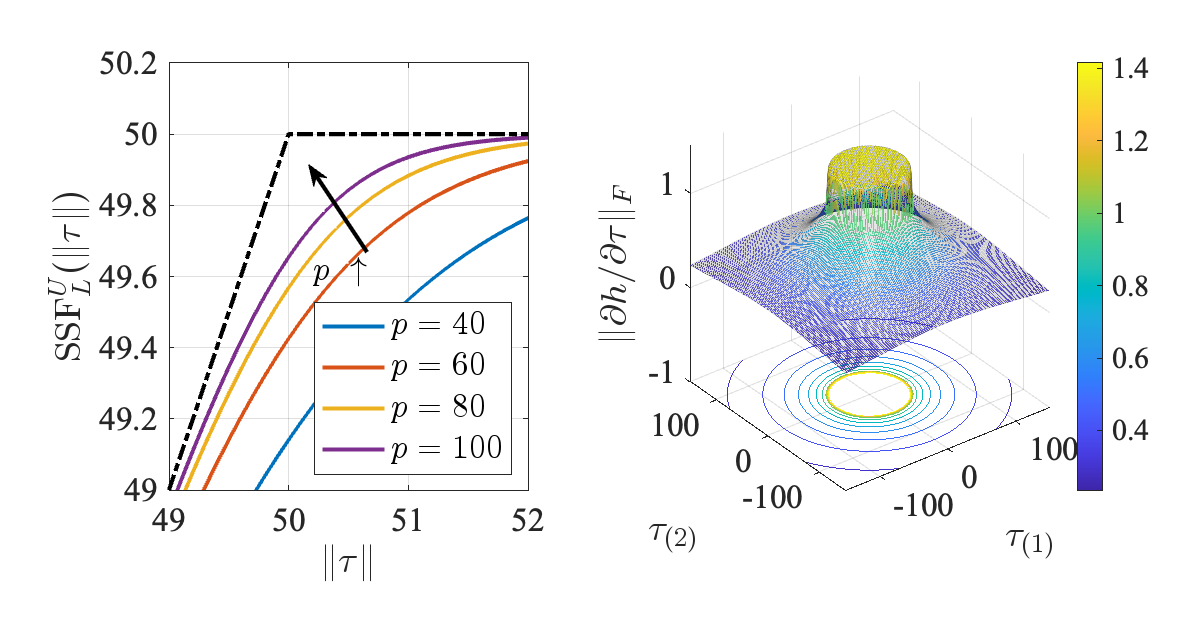
\includegraphics[width=0.9\linewidth]{fig/fig13.eps}
    \caption{Effect of parameter $p$ in the control input saturation function $h$ and boundedness of $\Vert\partial h/\partial \tau\Vert_F$.}
    \label{fig: h func}
\end{figure}

% SYSTEM FIGURE AND TABLE
% **********************************************************
Four controllers were examined for a comparative study. The first was the Backstepping Controller (BSC), used as the baseline. The second was the DNN-based Backstepping Controller (DNN-BSC), an existing neuro-adaptive control method where a DNN was employed to learn and compensate for the lumped system uncertainty function $f$ in the BSC. While this method addressed the weight norm constraint via a projection operator, it did not account for either the input norm or input bound constraints. The third was DNN-BSC augmented with an auxiliary system presented in \cite{RN55, RN56, RN3} (DNN-BSC-A), which handled the (linear) input saturation constraint but not the nonlinear input norm constraint. As a result, an approximation of the input norm constraint was used as an input bound constraint. Lastly, the proposed controller, CoNAC, rigorously considered system uncertainties, the weight norm constraint, and input constraints within a constrained optimization framework. The properties of these four controllers are summarized in Table \ref{table:controller}.
%and control input ball constraints presented in Appendix \ref{sec:cstr candidates}, included (named CoNAC).

\begin{table}[!t]
    \renewcommand{\arraystretch}{1.3}
    \caption{Properties of the controllers used in simulation}
    \label{table:controller}
    \centering
    \begin{tabular}{|c||c|c|c|}
    \hline
    & \multicolumn{3}{c|}{Handling Capability}\\
    \hline
    & System & Weight Norm & Input Norm\\
    &  Uncertainty & Constraint & Constraint\\
    \hline 
    BSC     & X & X & X\\
    \hline
    \multirow{2}{*}{DNN-BSC}     & \multirow{2}{*}{O} & O & \multirow{2}{*}{X}\\
         &  & (by projection) & \\
    \hline
    \multirow{2}{*}{DNN-BSC-A}   & \multirow{2}{*}{O} & O & $\triangle$ \\
       &  & (by projection) &  (by aux. system)\\
       % &  & & linearized constraint)\\
    % \hline
    % \multirow{3}{*}{DNN-BSC-A}   & \multirow{3}{*}{O} & O & $\triangle$ (by auxiliary\\
    %    &  & (by projection) &  system for \\
    %    &  & & linearized constraint)\\
    \hline
    \multirow{2}{*}{CoNAC}     &  \multirow{2}{*}{O} & O & O\\
         &  & (by optimization) & (by optimization)\\
    \hline
    \end{tabular}
\end{table}

% \begin{table}
% \caption{Specifications of the IPMSM Drive Used in the Experiment}\label{Tab3}
% \centering
% {\begin{tabular}{cc}\textcolor{black}ine
% \multicolumn{2}{c}{IPMSM}\\\textcolor{black}ine\textcolor{black}ine
% Rated power & 3 kW\\
% Rated speed & 4500 RPM\\
% Rated torque & 6.4 Nm\\
% Rotor inertia & 0.0021 kg$\cdot$m$^2$\\
% $I_{max}$ & 15 A \\
% $V_{dc}$ & 100 V\\
% $R_s$ & 0.34 $\Omega$\\
% $P$ & 3\\
% $T_s$ & 20 $\mu$s \\\textcolor{black}ine
% \multicolumn{2}{c}{Inverter}\\\textcolor{black}ine\textcolor{black}ine
% \multirow{2}{*}{Controller} & TMS320F28377D\\
% & (Texas Instrument) \\
% \multirow{2}{*}{IGBT module} & FS400R07A1E3\\
%  & (Infineon Technologies)
% \\\textcolor{black}ine
% \end{tabular}}
% \end{table}

% \begin{table}[!t]
%     \renewcommand{\arraystretch}{1.3}
%     \caption{Common Parameters of Selected Controllers.}
%     \label{table: error norm}
%     \centering
%     \begin{tabular}{|c||c|c|c|c|c|c|}
%     \hline
%     & $\alpha$ & ${k_q}$& ${k_z}$ & $M_0$ & $C_0$ & $G_0$ \\
%     \hline 
%     CM1 & - & 2 & 10 & $I_2$ & $I_2$ & $0_{2\times1}$\\
%     \hline
%     CM2 & 1e3 & 2 & 10 & $I_2$ & $I_2$ & $0_{2\times1}$\\
%     \hline
%     CM3 & 1e3 & 2 & 10 & $I_2$ & $I_2$ & $0_{2\times1}$\\
%     \hline
%     C & 1e3 & 2 & 10 & $I_2$ & - & -\\
%     \hline
%     \end{tabular}
%     \label{table: control parameters}
% \end{table}

% **** CM1,2 control law *****
The BSC used the control law defined in \eqref{eq. desired control} with $\hat f=[0,0]^\top$. Since BSC did not consider the unknown system dynamics, the approximation term $\hat f$ was set to zero.
%CM1 has the following control gains and design parameters: $k_s=5,{k_z}=5, M_0=I_2, C_0=I_2, G_0=[0,0]^\top  $.
% Since CM1 does not consider the unknown term, $\hat f$ was set to $[0,0]^\top$. 
The control law for DNN-BSC was the same as BSC, but the unknown system dynamics were approximated by a DNN \ie $\hat f\approx \hat\Phi$. The adaptation law for DNN-BSC, as presented in \cite{RN16}, was defined by 
\begin{equation}\label{eq:projection}
\dot {\hat\wth}= \text{Proj}_{\Omega}[\alpha  (\partial \hat\Phi/\partial \hat\wth)M_0^{-1}{\tilde z}],
\end{equation}
where $\text{Proj}_{\Omega}(\cdot)$ is the projection operator \cite[Appendix E, eq.~(E.4)]{RN20}, which projects an input vector onto a convex set $\Omega$. The convex set was defined as ${\Omega}\triangleq \{\Omega_0\,\cap\,\cdots\,\cap\, \Omega_k\}$, where $\Omega_i\triangleq \{\hat\wth_i\ \vert \ c_{b_i}\le 0\}, \ \forall i\in[0,\cdots, k]$, representing the weight norm constraint \eqref{eq. cstr weight ball}.
% The maximum control input ball constraint is not addressed since the stability analysis of \cite{RN16} uses the property that  $\text{Proj}_\Omega(\cdot)$ projects to the convex set, (\ie the constraints are generally non-convex on the $\hat\wth$-space.).
% **** CM3 control law *****

The control law for DNN-BSC-A was the same as DNN-BSC, but with an auxiliary system to compensate for control input violations. Since the auxiliary system handled only the input bound constraint, not the more complex input norm constraint \eqref{eq. cstr input ball}, an approximated version of the input norm constraint was used as an input bound constraint \eqref{eq. cstr input saturation} with ${\overline\tau_i} = -{\underline\tau_i} = (\bar\tau/\sqrt{2}+\bar\tau)/2$. The comparison between the original input norm constraint and its approximation is shown in Fig.~\ref{fig: ball control}.
%considering $h(\cdot)$, saturated control input is defined as $s(\tau)\triangleq \min(\max(\tau,-\bar\tau_s),\bar\tau_s)$, where $\bar\tau_s$ is $(\bar\tau/\sqrt{2}+\bar\tau)/2$;
The auxiliary system is defined as $\dot\zeta = A_\zeta \zeta + B_\zeta \Delta\tau,\quad \zeta\vert_{t=0} = 0$, where $\zeta\in\R^n$ denotes the auxiliary state, $A_\zeta=-[20,0;0;20],B_\zeta=[10,0;0,10]$, and $\Delta\tau_{(i)} = 
\tau_{(i)}-\text{sat}(\tau_{(i)},{\overline\tau_i},{\underline\tau_i})$
% s(\tau)-\tau$.
The auxiliary state variables were used in the adaptation law \eqref{eq:projection} by substituting ${\tilde z}$ with ${\tilde z}+\zeta$.

% **** CoNAC control law *****
The proposed CoNAC directly approximated the control law using the DNN as defined in \eqref{eq. approximated control}. The update rates for the multipliers were set as $\beta_{j}=0.1$. The weight matrix $W$ was selected as $W=\text{diag}([5,1,15,15])]$.

For all DNN-based controllers (DNN-BSC, DNN-BSC-A, and CoNAC), the DNN input vector $q_{NN}$ was set as the desired trajectory for ${q}$, \ie $q_{NN}=[{q_d}^\top,1]^\top$ with the augmented scalar 1 included to account for the bias term in the weight matrix. 
Each DNN architecture had two hidden layers with eight nodes (\ie $k=2, l_0=2, l_1=8, l_2=8, l_3=2$), and the adaptation gain was set to $\alpha =10^3$. The constraint parameters were $\bar\wth_0=20, \bar\wth_1=30, \bar\wth_2=40$, and $\bar\tau = 50$ (from Eq. \eqref{eq. h func}). The control parameters for all the controllers were set as ${k_q}=1.1,{k_z}=10,M_0=I_2,C_0=I_2,G_0=[0,0]^\top$.
The sampling time of the simulations was selected as $T_s=10^{-4}$.
% The same values were assigned across all the controllers for the common parameters for a fair comparison.
% The other parameters for CM1 to CoNAC were selected as listed in Table.~\ref{table: control parameters}. The same values were assigned across all the controllers for the common parameters for a fair comparison.

% **********************************************************
% SIMULATION FIGURES
\begin{figure*}[!t]
    \centering
        \subfloat[BSC]{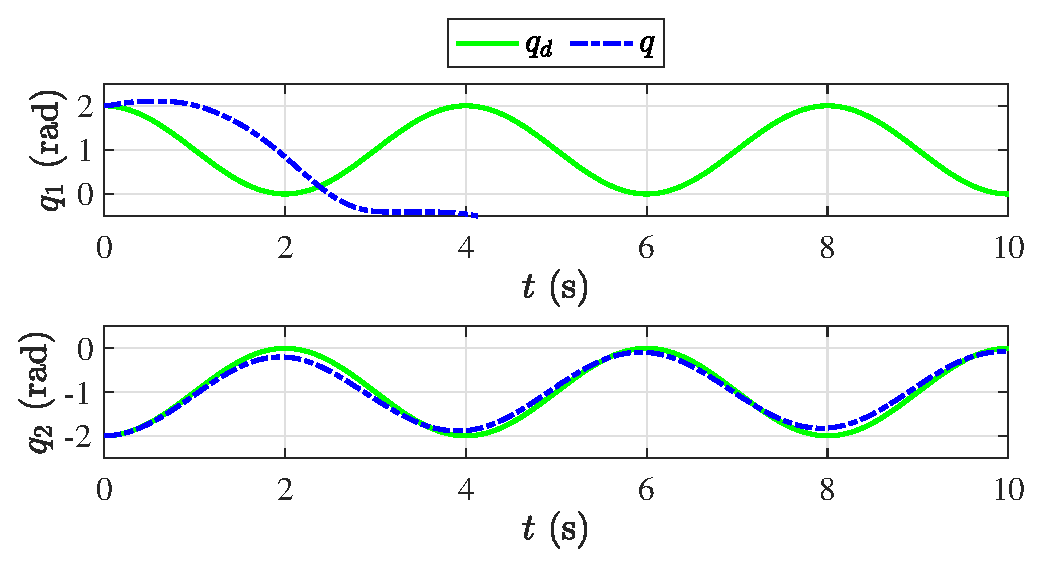
\includegraphics[width=0.49\linewidth]{fig/fig1.eps}%
        \label{fig: tracking_CM1}}
    \hfill
        \subfloat[DNN-BSC]{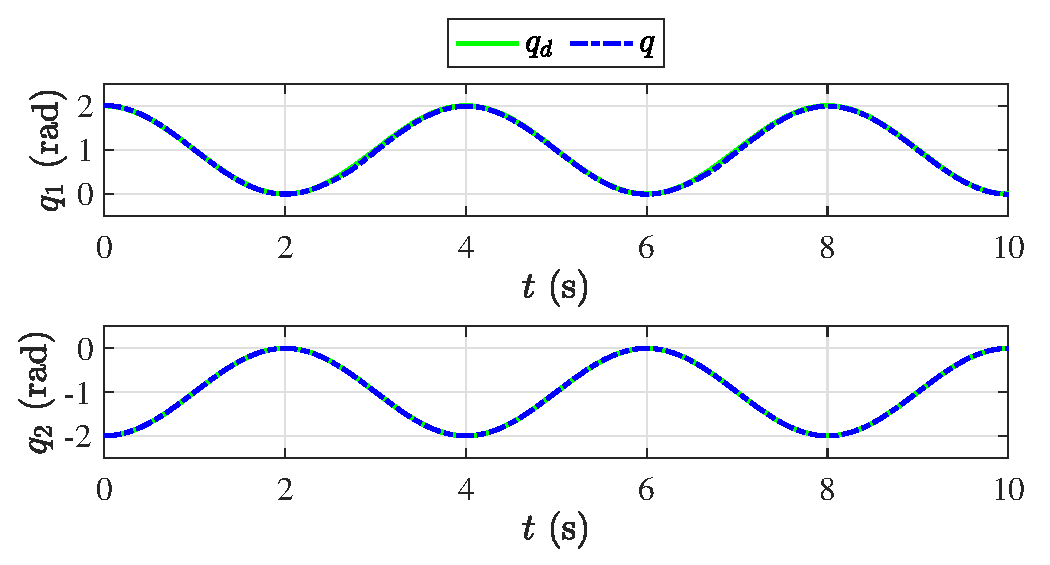
\includegraphics[width=0.49\linewidth]{fig/fig2.eps}%
        \label{fig: tracking_CM2}}
    \vfill
        \subfloat[DNN-BSC-A]{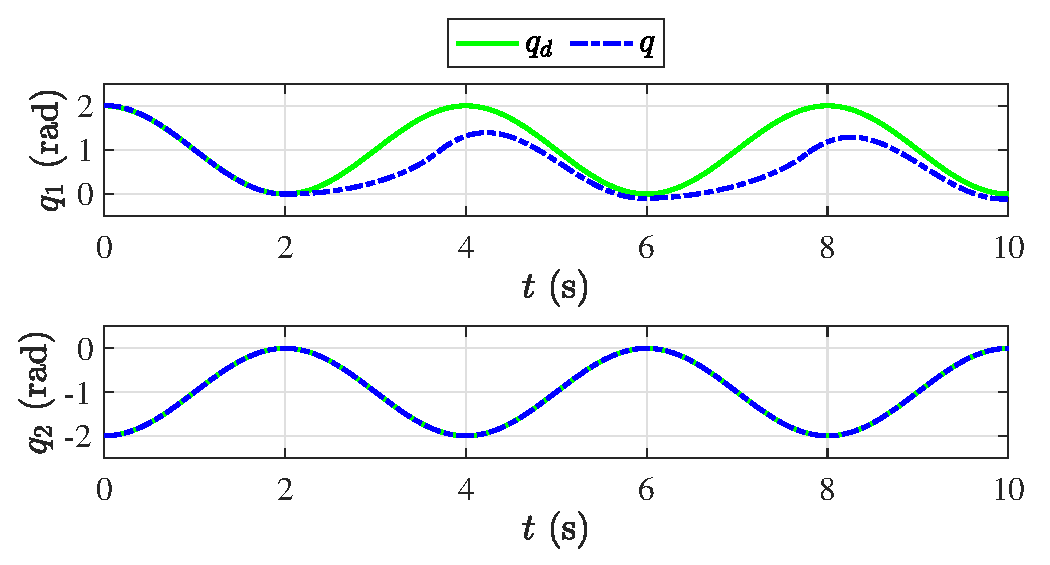
\includegraphics[width=0.49\linewidth]{fig/fig3.eps}%
        \label{fig: tracking_CM3}}
    \hfill
        \subfloat[CoNAC]{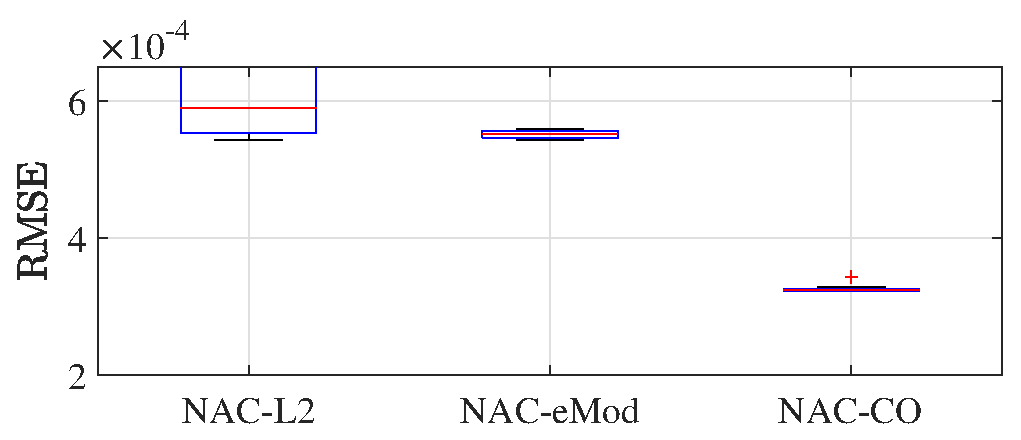
\includegraphics[width=0.49\linewidth]{fig/fig4.eps}%
        \label{fig: tracking_CoNAC}}
    \caption{Comparison of the tracking performance across the selected controllers.}
    \label{fig: tracking}
\end{figure*}

\begin{figure*}[!t]
    \centering
        \subfloat[BSC]{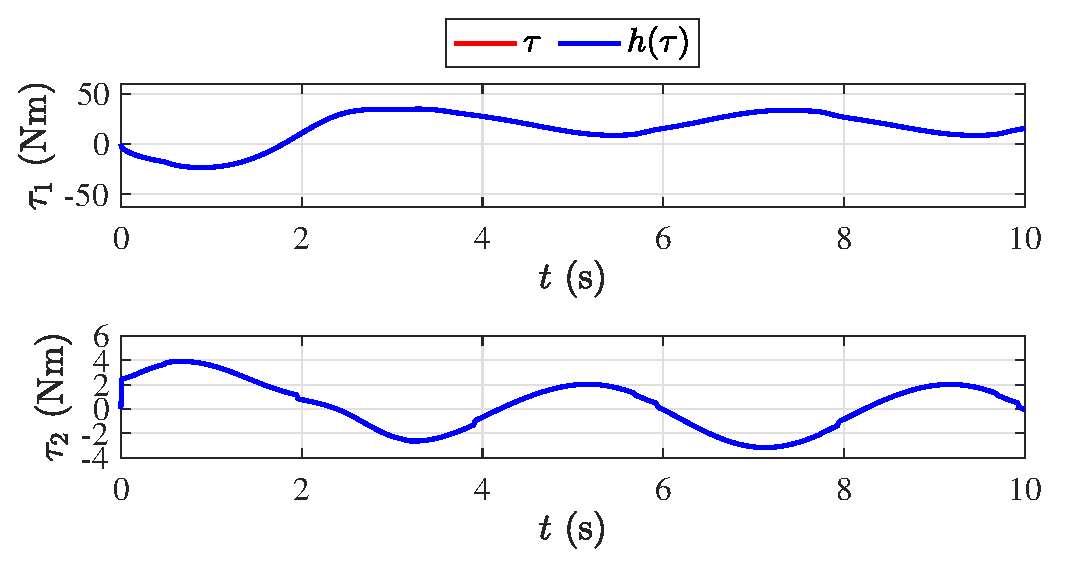
\includegraphics[width=0.49\linewidth]{fig/fig5.eps}%
        \label{fig: control_CM1}}
    \hfill
        \subfloat[DNN-BSC]{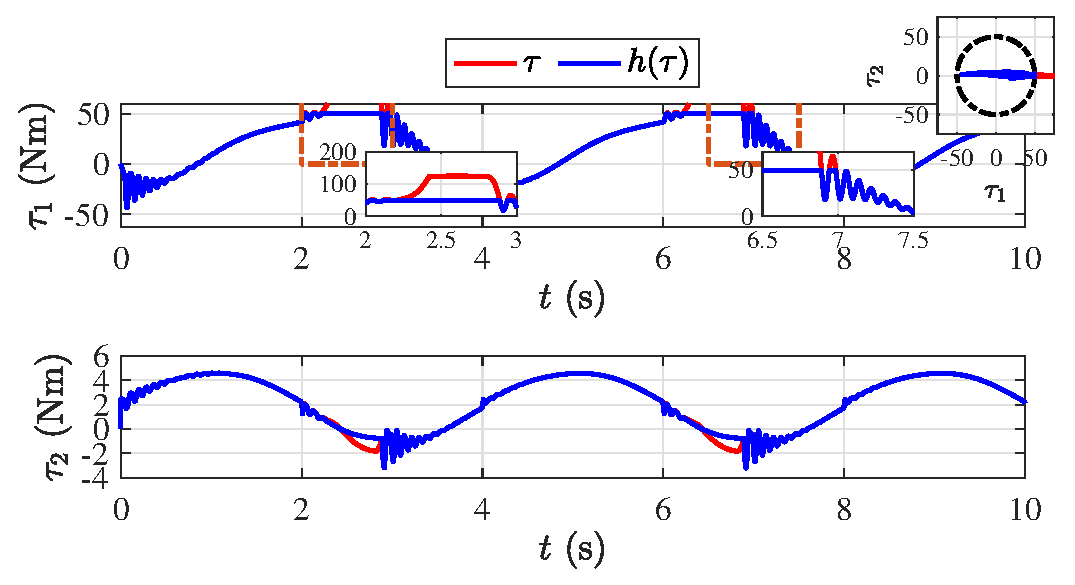
\includegraphics[width=0.49\linewidth]{fig/fig6.eps}%
        \label{fig: control_CM2}}
    \vfill
        \subfloat[DNN-BSC-A]{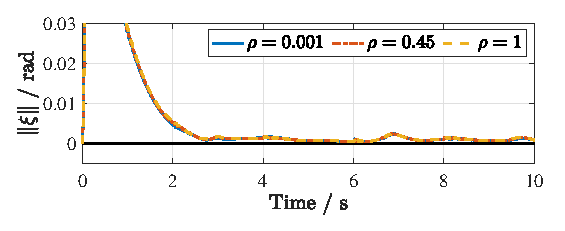
\includegraphics[width=0.49\linewidth]{fig/fig7.eps}%
        \label{fig: control_CM3}}
    \hfill
        \subfloat[CoNAC]{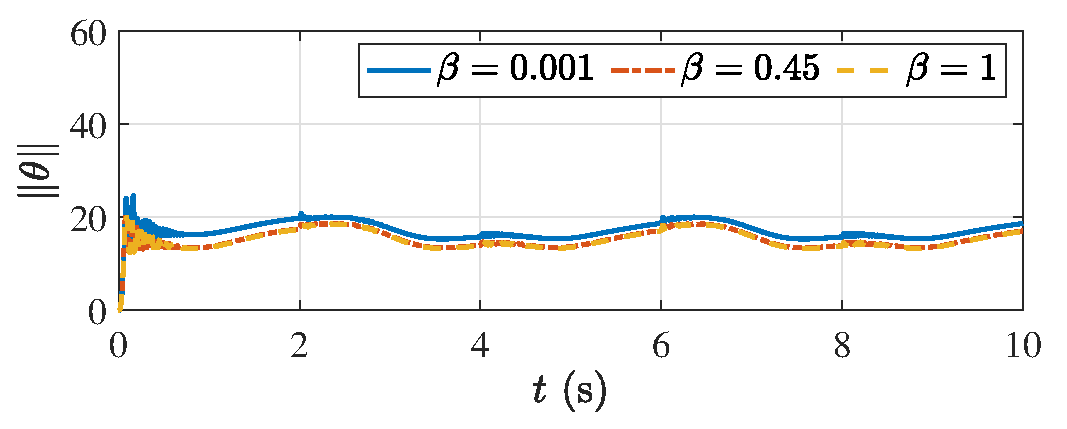
\includegraphics[width=0.49\linewidth]{fig/fig8.eps}%
        \label{fig: control_CoNAC}}
    \caption{Comparison of the control input $\tau$ and the physically saturated control input $h(\tau)$ across the selected controllers.}
    \label{fig: control}
\end{figure*}

\begin{figure}[!t]
    \centering
    {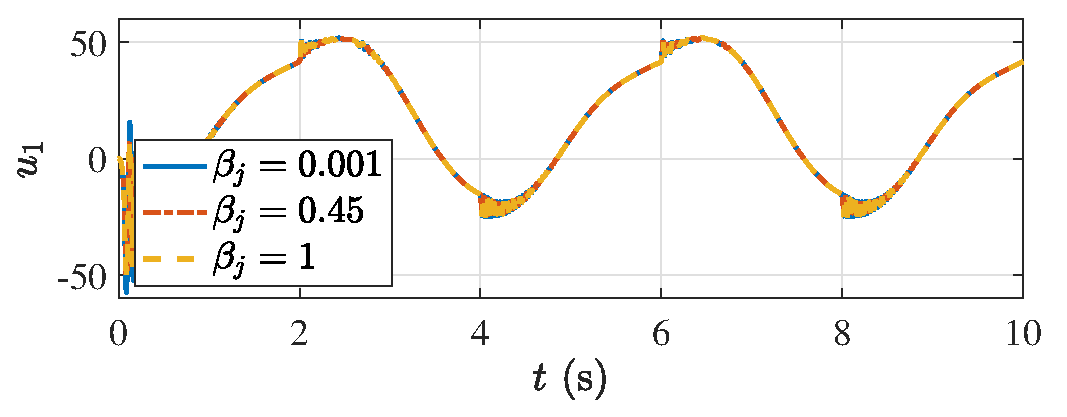
\includegraphics[width=0.9\linewidth]{fig/fig16.eps}
    \caption{Control input paths of DNN-BSC and CoNAC during the time interval from 5 s to 8 s.}
    \label{fig: ball control}}
\end{figure}

\begin{figure*}[!t]
    \centering
        \subfloat[Multipliers of CoNAC]{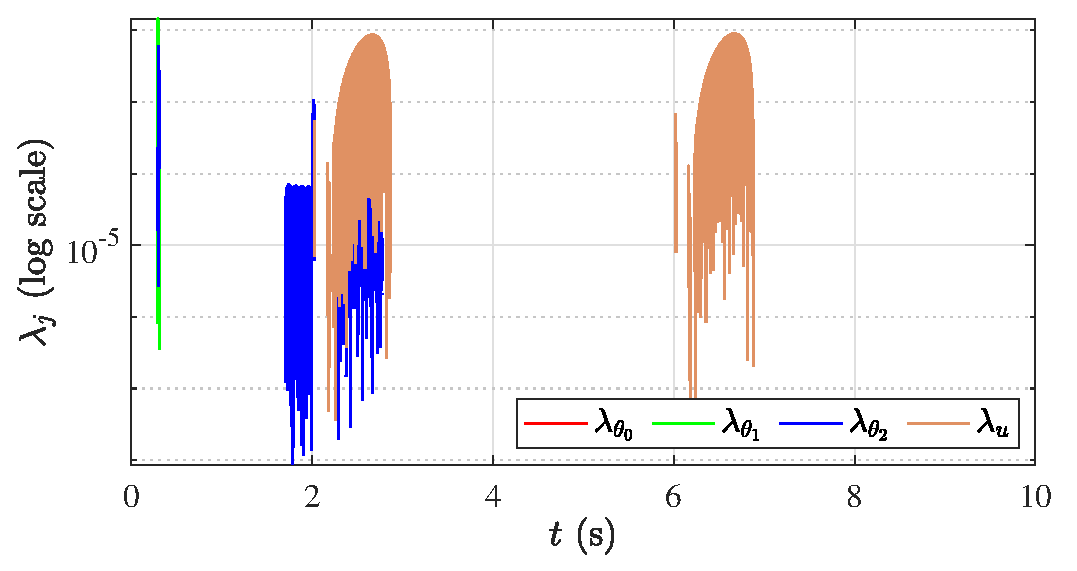
\includegraphics[width=0.49\linewidth]{fig/fig12.eps}%
        \label{fig: multiplier_CoNAC}}
    \hfill
        \subfloat[Weight norms of DNN-BSC]{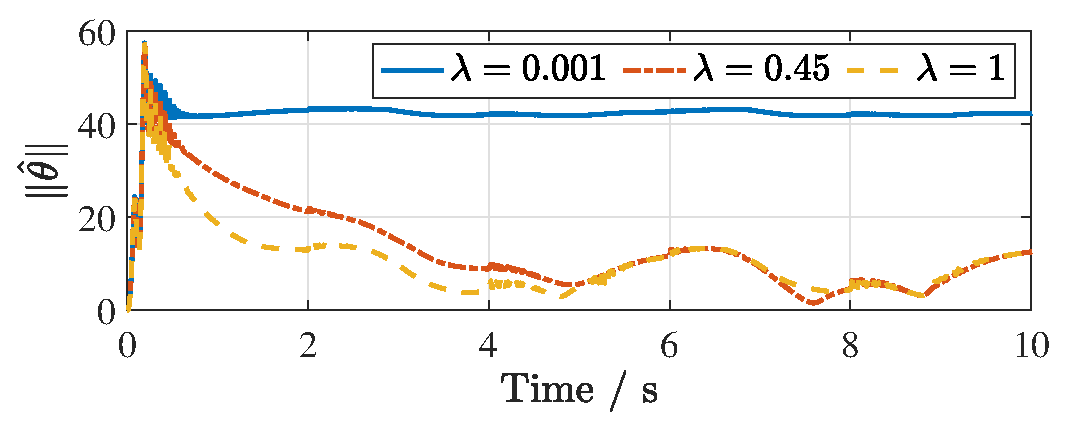
\includegraphics[width=0.49\linewidth]{fig/fig9.eps}%
        \label{fig: weight_CM2}}
    \vfill
        \subfloat[Weight norms of DNN-BSC-A]{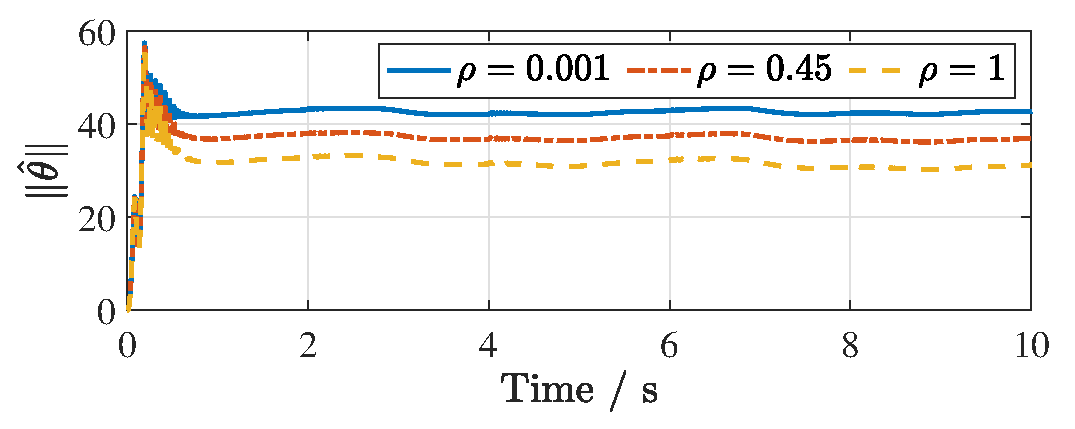
\includegraphics[width=0.49\linewidth]{fig/fig10.eps}%
        \label{fig: weight_CM3}}
    \hfill
        \subfloat[Weight norms of CoNAC]{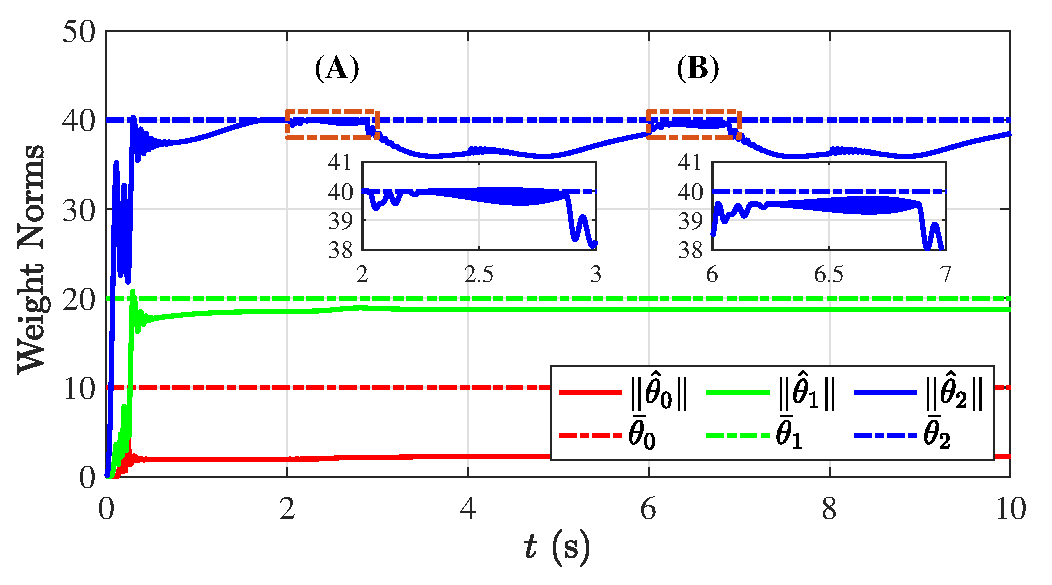
\includegraphics[width=0.49\linewidth]{fig/fig11.eps}%
        \label{fig: weight_CoNAC}}       
    \caption{Lagrange multipliers of CoNAC and weight norms of DNN-BSC, DNN-BSC-A, and CoNAC.}
    \label{fig: weight and multiplier}
\end{figure*}
% SIMULATION FIGURES
% **********************************************************

\subsection{System Uncertainty Handling}

The tracking results of the selected controllers are shown in Fig.~\ref{fig: tracking}.
To demonstrate the effectiveness of using DNNs for compensating the lumped system uncertainty function $f$, the gains ${k_q}$ and ${k_z}$ for BSC were intentionally selected as small values, resulting in a weak ability to handle these uncertainties. As a result,
%poor performance and sufficiently large values to satisfy \eqref{eq. ctrl stable condition}.
%the parameters of CM1 are poorly tuned, 
BSC failed to track the reference trajectory, as shown in Fig.~\ref{fig: tracking_CM1}.

By leveraging the DNN to compensate for the lumped system uncertainty within the BSC, DNN-BSC achieved improved tracking performance compared to BSC, as seen in Fig.~\ref{fig: tracking_CM2}. Fig.~\ref{fig: tracking_CM3} shows that DNN-BSC-A enhanced tracking performance for $q_2$, but tracking for $q_1$ remained unsatisfactory due to incomplete constraint handling, which will be discussed in detail in Section \ref{sec:sim_cnst}.
%By compensating the uncertain terms the control input of CM2 in Fig.~\ref{fig: control_CM2} is saturated.

Finally, CoNAC, which directly approximates the stabilizing control law along with the compensation term, demonstrated satisfactory tracking performance across both states, as illustrated in Fig.~\ref{fig: tracking_CoNAC}.

\subsection{Input Norm Constraint Handling}\label{sec:sim_cnst}

The resulting control input $\tau$ and physically saturation control input $h(\tau)$ for the selected controllers are shown in Fig.~\ref{fig: control}. As illustrated in Fig.~\ref{fig: control_CM1}, BSC did not violate the input norm constraint (\ie $\tau = h(\tau)$). However, in DNN-BSC, the added compensation term from the DNN caused violations of the input norm constraint (\ie $\tau > h(\tau)$) at several points; see Fig.~\ref{fig: control_CM2}. This failure to account for the input norm constraint led to oscillations in the control input $\tau$. The DNN adaptation process attempted to increase the weights to reduce the residual errors that were not constrained by saturation, but after saturation ceased, the control input had to rapidly adjust back to realistic levels, leading to oscillatory behavior. Such high-frequency oscillations may induce instability in the control system or cause fatigue in the actuators.

On the other hand, both DNN-BSC-A and CoNAC successfully handled their imposed input constraints, as shown in Fig.~\ref{fig: control_CM3} and Fig.~\ref{fig: control_CoNAC}, respectively, without causing notable oscillations in the control input $\tau$ even after the input constraint was activated. However, the tracking performance of DNN-BSC-A was lower than that of DNN-BSC and CoNAC, as the auxiliary system used in DNN-BSC-A approximated the input norm constraint with an input bound constraint, creating a rectangular constraint in the $\tau$-space (see Fig.~\ref{fig: ball control}). In contrast, CoNAC satisfied the nonlinear input norm constraint and produced the physically maximum control input, resulting in improved tracking performance. 

It is also important to note that the control input trajectory in DNN-BSC-A depends on the dynamics of the auxiliary system. The auxiliary system regulates the violated control input after sufficient auxiliary state $\zeta$ is generated to compensate for the violation. This can be observed in Fig.~\ref{fig: ball control}, where DNN-BSC-A exhibited minor violations of the input bound constraint. In contrast, CoNAC satisfied the constraint without being affected by such dynamics, as its Lagrange multiplier adjusted as soon as the constraint was violated.

%Meanwhile, CM2 and CM3 is based on BSC, and the desired controller $\tau^*$ of CoNAC is based on the BSC which may produce larger control input by canceling the stabilizing system dynamics.
%Therefore, CM2, CM3, and CoNAC produced the saturated control input.
%These control results show why the control saturation should be handled.

\subsection{Weight Norm Constraint Handling}

The resulting weight norms of DNN-BSC, DNN-BSC-A, and CoNAC, along with the Lagrange multipliers of CoNAC, are shown in Fig.~\ref{fig: weight and multiplier}. All three controllers—DNN-BSC, DNN-BSC-A, and CoNAC—maintained weight norms within the imposed weight norm constraints.

IN DNN-BSC, as shown in Fig.~\ref{fig: weight_CM2}, the weight norm of the last layer (\ie $\Vert {{{\hat \wth }_2}} \Vert$) fluctuated significantly over time, proportional to the control input norm. This is because the last layer’s weights directly determine the control input. When the control input violated the input norm constraint, the last layer’s weight norm hit the boundary and stayed there due to the projection operator. However, the projection operator only responded to violations without considering optimality or behavior.
%In the case of CM2 which does not consider the control input constraint, the weight norm of the last layer reaches the maximum weight norm value, when the control is saturated.
%It is because the weights get increased to produce larger control input to reduce the tracking error of $q_2$. (\ie the maximum magnitude of the control input depends on the weight norm of the last layer, since the activation function is bounded.)

In DNN-BSC-A, none of the weight norms reached their boundaries, as shown in Fig.~\ref{fig: weight_CM3}. This was due to the auxiliary system, where the auxiliary state $\zeta$ reduced the control input, ensuring it stayed within the input constraint.

In CoNAC, all weight norms complied with the imposed constraints through the constrained optimization approach, as illustrated in Fig.\ref{fig: weight_CoNAC}. When any weight norm approached its upper limit, the Lagrange multiplier was promptly activated to steer the weight adaptation direction towards a constraint-satisfactory point (see Fig.\ref{fig: multiplier_CoNAC}). Notably, the weight norms of the first and second layers ($\Vert {{{\hat \wth }_0}} \Vert$ and $\Vert {{{\hat \wth }_1}} \Vert$) remained nearly constant throughout the control period. The weight norm of the last layer $\Vert {{{\hat \wth }_2}} \Vert$ stabilized within the upper bound by around 6.5 seconds (see Fig.~\ref{fig: weight_CoNAC} (B)), coinciding with the activation of the input norm constraint. This quasi-static behavior of the weight norm (\ie $d{\hat\wth}/dt=-\alpha\partial L/\partial \hat\wth \approx 0$) along with the quasi-static behavior of the Lagrange multipliers (\ie $\dot\lambda_j = \beta_j c_j \approx 0$) implies that the weights were updated near the KKT conditions, signifying local optimality in CoNAC. However, at around 2.5 seconds (see Fig.~\ref{fig: weight_CoNAC} (A)), the weight norm of the last layer reached the upper limit earlier, despite similar control conditions as the case at 6.5 seconds. This earlier saturation likely occurred because the optimization process had not yet fully converged to the optimal weight values.
%(\ie $\partial J/\partial\hat\wth = \sum_{j\in\mathcal {A}}\lambda_j\nabla_{\hat\wth} c_j)$.
%, by the multipliers increased due to the violation of the constraints as shown in Fig.~\ref{fig: multiplier_CoNAC}.

The overall weight norms of CoNAC were larger than those of DNN-BSC and DNN-BSC-A, since CoNAC approximated the entire stabilizing control law, whereas DNN-BSC and DNN-BSC-A only approximated the system uncertainty term within the BSC framework.

%Because the simulation is implemented in a digital computer, the multipliers repeat to disappear and be generated, since the constraints are satisfied and violated in the digital process.

%\subsection{Analysis of the Neural Network}

%Generally, the existing literature states that the maximum norms of the weights should be sufficiently large (\ie $\bar\wth_i \gg 0$) since the designer does not know where the global optimal point of the weights is.
%However, using the physical prior knowledge of the system, one can guess the proper value of the maximum norm, since the magnitude of the control input depends on the last layer's weights due to the bounded activation function.
%Furthermore, the simulation study shows that the selected controllers have sufficiently good performances with the small maximum weight norms.
%It means that the local optimal point of the weights are more effective for the stability analysis and the limitating the control input's amplitude.

%Since it is generally known that the deeper NNs have better approximation performance with less computation cost, the NNs should have more layers.
%However, because the NNs in this paper utilize $\tanh(\cdot)$ as the activation function, the NNs have the gradient vanishing problem as shown in Fig.~\ref{fig: weight_CM2}-\ref{fig: weight_CoNAC}. (\ie the weight updates are smaller as its layer is closer to the input layer.)
%To address this issue, the activation function should be selected as the ReLU or the Leaky ReLU, while ensuring the stability of the controller.

%  SECTION CONCLUSION ======================================
\section{Conclusion}\label{sec:conclusion}

This paper presented a constrained optimization-based neuro-adaptive controller (CoNAC) for the uncertain Euler-Lagrange system, addressing both weight norm and input constraints through a rigorous optimization framework. The stability of the proposed controller was analyzed using Lyapunov theory, ensuring that the system maintained bounded tracking and estimation errors under real-time adaptation.

The controller effectively incorporated both the input (bound or norm) constraint and the weight norm constraint, ensuring that both actuator limitations and neural network weights were kept within predefined bounds. By formulating these constraints as part of the optimization process, CoNAC ensured that the weights converged in a way that satisfied the Karush-Kuhn-Tucker (KKT) conditions, guaranteeing optimality and stability.

Simulation results validated the superior performance of CoNAC compared to conventional methods, such as DNN-BSC and DNN-BSC-A. CoNAC not only handled complex input constraints but also managed the weight norm constraints rigorously, leading to improved tracking accuracy and stability without notable oscillations.

Future work may extend this approach to address constraints on both the system inputs and states, further enhancing the flexibility and robustness of neuro-adaptive control systems using constrained optimization.

%  BIBLIOGRAPHY ============================================
\bibliographystyle{ieeetr}
\bibliography{refs}

\end{document}
